\section{Continuous Probability}
We will focus on the case where $\operatorname{Im}(X)$ is an \underline{interval} in $\mathbb{R}$.\\
\underline{Why?}
\begin{itemize} \color{blue}
    \item Natural for measuring physical quantities, proportions \dots
    \item ``Limits'' of discrete RV.
    \item Calculus tools for nice calculations.
\end{itemize} 

\begin{definition}[Random Variable - Redefintion]
    A \vocab{random variable} $X$ on $(\Omega, \mathcal{F}, \mathbb{P})$ is a function $X : \Omega \to \mathbb{R}$ s.t. ${X \leq x} \in \mathcal{F}$.
\end{definition} 
This is consistent with the previous definition when $\Omega$ is countable (or $\operatorname{Im}(X)$ is countable).

\underline{Drawback}: We cannot take $\mathcal{F} = \mathcal{P}(\mathbb{R})$.

\begin{definition}[Cumulative Distribution Function]
    The \vocab{cdf} of RV $X$ is
    \begin{align*}
        F_X: \mathbb{R} &\to [0, 1] \\
        F_X(x) &= \mathbb{P}(X \leq x).
    \end{align*} 
\end{definition} 

\begin{example}[A 6-sided dice]
ars
\end{example} 

\subsection{Properties of CDF}

\begin{claim}
    $F_X$ increasing i.e. $x \leq y \implies F_X(x) \leq F_y(y)$.
\end{claim} 

\begin{proof}
    $F_X(x) = \mathbb{P}(X \leq x) \leq \mathbb{P}(X \leq y) = F_X(y)$.
\end{proof} 

\begin{claim}
    $\mathbb{P}(X > x) = 1 - F_X(x)$
\end{claim} 

\begin{claim}
    $\mathbb{P}(a < X \leq b) = F_X(b) - F_X(a)$
\end{claim} 

\begin{proof}[Proof (Not Lectured)]
    \begin{align*}
        \mathbb{P}(a<X\leq b) &= \mathbb{P}(\{a<X\}\cap \{X\leq b\}) \\
        &=\mathbb{P}(X\leq b) - \mathbb{P}(\{X\leq b\}\cap \{X\leq a\}) \\
        &=\mathbb{P}(X\leq b) - \mathbb{P}(X\leq a)
    \end{align*}
\end{proof}

\begin{claim}
    $F_X$ is right-continuous and the left limit exists, i.e. $\lim_{y \downarrow x} F_X(y) = F_X(x)$ and $\lim_{y \uparrow x} F_X(y) = F_X(x -) = \mathbb{P}(X < x)$.
\end{claim} 

\begin{proof}[Proof - Right Continuous]
    STP $F_X \left(x + \frac{1}{n}\right) \to F_X(x)$ as $n \to \infty$. \\
    Let $A_n = \{x<X\leq x+\frac{1}{n}\}$.
    Then $(A_n)$ are decreasing events and $\bigcap_n A_n = \emptyset$. \\
    So $\mathbb{P}(A_n) = F_X \left(x + \frac{1}{n}\right) - F_X(x)$ and $\mathbb{P}(A_n) \to \mathbb{P}(\emptyset) = 0$.
\end{proof} 

\begin{proof}[Proof - Left Limits]
    $F_X \left(x - \frac{1}{n}\right)$ is an increasing sequence bounded above by $F_X(x)$. \\
    Consider $B_n = \left\{X \leq x - \frac{1}{n}\right\}$ then $(B_n)$ increasing and $\bigcup_n B_n = \{X < x\}$.
    So $F_X \left(x - \frac{1}{n}\right) = \mathbb{P}(B_n) \to \mathbb{P}(X < x)$.
\end{proof} 

\begin{claim}
    $\lim_{x \to \infty} F_X = 1$, $\lim_{x \to - \infty} F_X = 0$.
\end{claim} 

\begin{proof}
    Let $A_n = {X \leq n}$, so $(A_n)$ are increasing events and $\cup_n A_n = \Omega$.
    So $F_X(n) = \mathbb{P}(X \leq n) \to \mathbb{P}(\Omega) = 1$ by \nameref{prp:continuity}.

    Similar for $\lim_{x \to - \infty} F_X = 0$.
\end{proof} 

\subsection{Continuous RVs}
\begin{definition}[Continuous RV]
    A RV is \vocab{continuous} if $F$ is continuous.
\end{definition} 

\begin{claim}
    If $X$ is a continuous RV then $\mathbb{P}(X = x) = 0 \quad \forall \; x$.
\end{claim} 

\begin{proof}
    \begin{align*}
        F_X(x) &= F_X(x-) \\
        \iff \mathbb{P}(X \leq x) &= \mathbb{P}(X < x) \quad \forall \; x \\
        \iff \mathbb{P}(X = x) &= 0 \quad \forall \; x.
    \end{align*} 
\end{proof} 

\begin{note}
    In this course we assume that $F$ is also differentiable so that $F_X(x) = \mathbb{P}(X \leq x) = \int_{-\infty}^{x} f_X(u) \,du$.
\end{note} 

\begin{definition}[Probability Density Function]
    The \vocab{pdf} of RV $X$ is $f_X : \mathbb{R} \to \mathbb{R}$ with properties
    \begin{align*}
        f_X(x) &\geq 0 \quad \forall \; x \\
        \int_{-\infty}^{\infty} f_X(x) \,dx &= 1.
    \end{align*} 
\end{definition} 

\underline{Intuitive meaning}
\begin{align*}
    \mathbb{P}(x < X \leq x + \delta x) &= \int_{x}^{x + \delta x} f_X(u) \,du \approx \delta x \cdot f_X(x) \\
    \mathbb{P}(a < X \leq b) &= \int_{a}^{b} f_X(x) \,dx \\
    &= \mathbb{P}(a \leq X < b) \color{red} \text{ since } \mathbb{P}(X = a) = \mathbb{P}(X = b) = 0.
\end{align*} 

\tikzset{every picture/.style={line width=0.75pt}} %set default line width to 0.75pt        

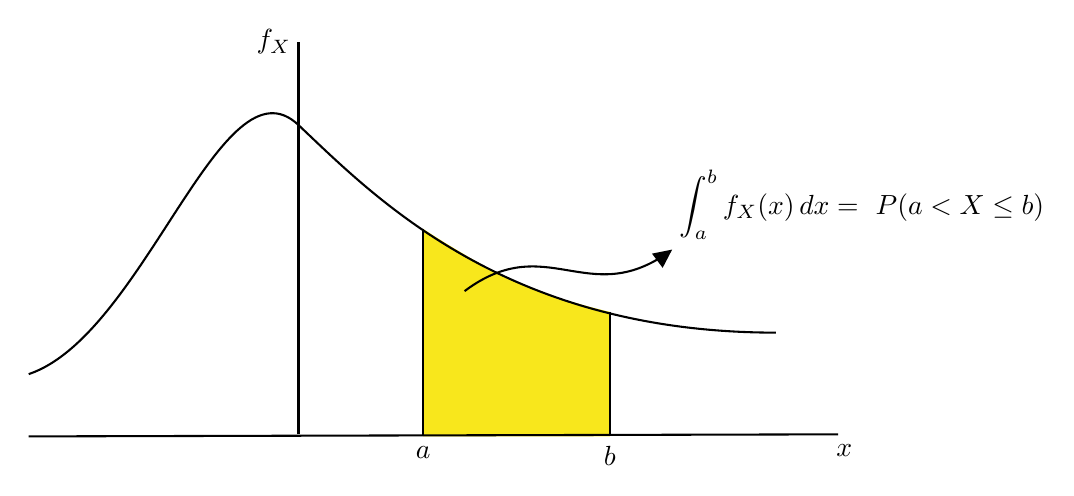
\begin{tikzpicture}[x=0.75pt,y=0.75pt,yscale=-1,xscale=1]
%uncomment if require: \path (0,300); %set diagram left start at 0, and has height of 300

%Shape: Polygon Curved [id:ds9211984515564444] 
\draw  [draw opacity=0][fill={rgb, 255:red, 248; green, 231; blue, 28 }  ,fill opacity=1 ] (230,140) .. controls (230,140) and (262,161) .. (280,168) .. controls (298,175) and (320,180) .. (320,180) .. controls (320,180) and (320,240) .. (320,240) .. controls (320,240) and (230,240) .. (230,240) .. controls (230,240) and (230,140) .. (230,140) -- cycle ;
%Straight Lines [id:da9217955375911691] 
\draw    (40,240) -- (430,239) ;
%Curve Lines [id:da17179804759111184] 
\draw    (40,210) .. controls (96,191) and (133,55) .. (170,90) .. controls (207,125) and (270,190) .. (400,190) ;
%Straight Lines [id:da4200417602105906] 
\draw    (230,140) -- (230,240) ;
%Straight Lines [id:da5043108171804249] 
\draw    (320,180) -- (320,240) ;
%Straight Lines [id:da456272514459267] 
\draw    (170,239) -- (170,50) ;
%Curve Lines [id:da08440500141214824] 
\draw    (250,170) .. controls (289.2,140.6) and (309.19,178.43) .. (347.62,151.72) ;
\draw [shift={(350,150)}, rotate = 503.13] [fill={rgb, 255:red, 0; green, 0; blue, 0 }  ][line width=0.08]  [draw opacity=0] (8.93,-4.29) -- (0,0) -- (8.93,4.29) -- cycle    ;

% Text Node
\draw (433,242.4) node [anchor=north] [inner sep=0.75pt]    {$x$};
% Text Node
\draw (168,50) node [anchor=east] [inner sep=0.75pt]    {$f_X$};
% Text Node
\draw (230,243.4) node [anchor=north] [inner sep=0.75pt]    {$a$};
% Text Node
\draw (320,243.4) node [anchor=north] [inner sep=0.75pt]    {$b$};
% Text Node
\draw (352,146.6) node [anchor=south west] [inner sep=0.75pt]    {$\displaystyle \int_{a}^{b} f_X(x) \,dx =\ \mathbb{P}( a< X\leq b)$};


\end{tikzpicture}

So for $S \subset \mathbb{R}$, $\mathbb{P}(X \in S) = \int_{S} f_X(u) \,du$. \color{blue} ($S$ ``nice'' e.g. interval or countable union of intervals) \color{black}

\underline{Key takeaways}:
\begin{itemize}
    \item The CDF is a collection of probabilities
    \item The PDF is \underline{not} a probability. We use them by integrating to get a probability.
\end{itemize} 

\begin{example}[Uniform Distribution]
    Let $X \sim \operatorname{U}[a, b]$ where $a, b \in \mathbb{R}$ and $a < b$.
    \begin{align*}
        f_X(x) &= \begin{cases}
            \frac{1}{b - a} & x \in [a, b] \\
            0 & \text{otherwise}
        \end{cases} \\
        F_X(x) &= \int_{a}^{x} f_X(u) \,du \\
        &= \frac{x - a}{b - a} \ \text{ for } a \leq x \leq b.
    \end{align*} 
\end{example} 

\begin{question}
    \color{blue} In what sense is this a ``limit of discrete uniform RVs''?
\end{question} 

\begin{example}[Exponential Distribution]
    Let $X \sim \operatorname{Exp}(\lambda)$ where $\lambda > 0$.
    \begin{align*}
        f_X(x) &= \begin{cases}
            \lambda e^{- \lambda x} & x > 0 \\
            0 & \text{otherwise}
        \end{cases}
        \intertext{It is easy to check that $f_X(x)$ is a pdf.}
        F_X(x) &= \mathbb{P}(X \leq x) \\
        &= \int_{0}^{x} \lambda e^{-\lambda u} \,du \\
        &= 1 - e^{- \lambda x}.
    \end{align*} 
\end{example} 

\color{blue} The exponential distribution is the ``limit of (rescaled) geometric distribution''.
It is a good way to model \underline{arrival times}, ``how long to wait before something happens'' - \color{red} link to Poisson usage which will be explored in Part II. \color{black}

\begin{claim}[Memoryless property]
    (Conditional $\mathbb{P}$ works as before).
    Let $X \sim \operatorname{Exp}(\lambda)$ and $s, t > 0$.
    \begin{align*}
        \mathbb{P}(X \geq s + t \mid X \geq s) &= \mathbb{P}(X \geq t).
    \end{align*} 
\end{claim} 

\begin{proof}
    \begin{align*}
        \mathbb{P}(X \geq s + t \mid X \geq s) &= \frac{\mathbb{P}(X \geq s + t)}{\mathbb{P}(X \geq s)} \\
        &= \frac{e^{-\lambda(s + t)}}{e^{-\lambda s}} \\
        &= e^{-\lambda t} \\
        &= \mathbb{P}(X \geq t).
    \end{align*} 
\end{proof} 

\begin{note}
    The only continuous memoryless distribution (with a density) is the exponential distribution.
\end{note} 

\subsection{Expectation of Continuous RVs}
\begin{definition}[Expectation]
    The \vocab{expectation} of $X$ is $\int_{-\infty}^{\infty} x f_X(x) \,dx$ and $\mathbb{E}[g(X)] = \int_{-\infty}^{\infty} g(x) f_X(x) \,dx$.\footnote{\color{blue} Technical comment: assumes at most one of $\int_{-\infty}^{0} |x| f_X(x) \,dx$ and $\int_{0}^{\infty} x f_X(x) \,dx$ is infinite.}
\end{definition} 

\begin{claim}[Linearity of Expectation]
    $\mathbb{E}[\lambda X + \mu Y] = \lambda \mathbb{E}[X] + \mu \mathbb{E}[Y]$.
\end{claim} 

\begin{claim}
    If $X \geq 0$ then $\mathbb{E}[X] = \int_{0}^{\infty} \mathbb{P}(X \geq x) \,dx$.
\end{claim} 

\begin{proof}
    \begin{align*}
        \mathbb{E}[X] &= \int_{0}^{\infty} x f_X(x) \,dx \\
        &= \int_{\mathcolor{blue}{x=0}}^{\color{blue} \infty} \left( \int_{\mathcolor{red}{u = 0}}^{\color{red} x} 1 \,du \right) f_X(x) \,dx \\
        &= \int_{\mathcolor{red}{u = 0}}^{\color{red} \infty} \,du \int_{\mathcolor{blue}{x = u}}^{\color{blue} \infty} f_X(x) \,dx\footnote{Consider the region of $(u, x)$ space the second line integrates over and see this is the same as the third line.} \\
        &= \int_{\mathcolor{red}{u = 0}}^{\color{red} \infty} \,du \color{blue} \mathbb{P}(X \geq u)
    \end{align*} 
\end{proof} 

\subsection{Variance of Continuous RVs}
\begin{definition}[Variance]
    $\Var(X) = \mathbb{E} \left[(X - \mathbb{E}[X])^2 \right] = \mathbb{E} \left[X^2 \right] - (\mathbb{E}[X])^2$.
\end{definition} 

\begin{claim}
    $\Var(aX + b) = a^2 \Var(X)$.
\end{claim} 

\begin{example}[Uniform Distribution]
    Let $X \sim \operatorname{U}[a, b]$.
    \begin{align*}
        \mathbb{E}[X] &= \int_{a}^{b} x \frac{1}{b - a} \,dx \\
        &= \frac{a + b}{2} \\
        \mathbb{E}[X^2] &= \int_{a}^{b} x^2 \frac{1}{b - a} \,dx \\
        &= \frac{1}{3} \left( a^2 + ab + b^2 \right) \\
        \Var(X) &= \frac{1}{3} \left( a^2 + ab + b^2 \right) - \left( \frac{a + b}{2} \right)^2 \\
        &= \frac{(b - a)^2}{12}.
    \end{align*} 
\end{example} 

\begin{example}[Exponential Distribution]
    Let $X \sim \operatorname{Exp}(\lambda)$.
    \begin{align*}
        \mathbb{E}[X] &= \int_{0}^{\infty} x \lambda e^{- \lambda x} \,dx \\
        &= \left[ - x e^{- \lambda x}\right]_0^\infty + \int_{0}^{\infty} e^{- \lambda x} \,dx \\
        &= \frac{1}{\lambda}. \\
        \mathbb{E}[X^2] &= \int_{0}^{\infty} x^2 \lambda e^{- \lambda x} \,dx \\
        &= \left[ - x^2 e^{- \lambda x}\right]_0^\infty + 2 \int_{0}^{\infty} x e^{- \lambda x} \,dx \\
        &= 0 + \frac{2}{\lambda^2}. \\
        \Var(X) &= \frac{2}{\lambda^2} - \frac{1}{\lambda^2} \\
        &= \frac{1}{\lambda^2}.
    \end{align*} 
\end{example} 

\subsection{Transformations of Continuous RVs}

Goal: \begin{itemize}
    \item Let $U \sim \operatorname{Unif}[a, b]$ and $\tilde{U} \sim \operatorname{Unif}[0, 1]$. We want to be able to write $U = (b - a) \tilde{U} + a$ and carry all calculations over.
    \item View $g(X)$ as a continuous RV with its own density.
\end{itemize} 

\begin{theorem} \label{theorem:transrv} ~\vspace*{-1.5\baselineskip}
    \begin{itemize}
        \item Let $X$ be a continuous RV with density $f$. 
        \item Let $g: \mathbb{R} \to \mathbb{R}$ be continuous s.t.
        \begin{itemize}
            \item $g$ is either strictly increasing or strictly decreasing.
            \item $g^{-1}$ is differentiable.
        \end{itemize} 
    \end{itemize} 
    Then $g(X)$ is a continuous RV with density
    \begin{align}
        \hat{f}(x) = f(g^{-1}(x)) \cdot \left|\frac{d}{dx} g^{-1}(x)\right| \label{align*:transrv}
    \end{align} 
\end{theorem}

\begin{remark} ~
    \begin{itemize}
        \item Density is? Something to integrate over to get a probability.
        \item \Cref{align*:transrv} \underline{is} integration by substitution.
        \item The following proof uses CDFs (which \underline{are} probabilities).
    \end{itemize} 
\end{remark} 

\begin{proof}
    \color{red} Assume $g$ is strictly increasing, $g$ strictly decreasing case is similar. \color{black}
    \begin{align*}
        F_{g(X)}(x) &= \mathbb{P}(g(X) \leq x) \\
        &= \mathbb{P}(X \leq g^{-1}(x)) \\
        &= F_X(g^{-1}(x)) \\
        F_{g(X)}'(x) &= F_X'(g^{-1}(x)) \frac{d}{dx} g^{-1}(x) \\
        &= f(g^{-1}(x)) \frac{d}{dx} g^{-1}(x).
    \end{align*} 
\end{proof}

\underline{Sanity check}: We've got two expressions for $\mathbb{E}[g(X)]$, $\int_{-\infty}^{\infty} x \hat{f}(x) \,dx$ and $\int_{-\infty}^{\infty} g(x) f(x) \,dx$. 
\color{blue} (Assume $\operatorname{Im}(X) = \operatorname{Im}(g(X)) = (- \infty, \infty)$). \color{black}

\begin{align*}
    \int_{-\infty}^{\infty} x \hat{f}(x) \,dx &= \int_{-\infty}^{\infty} x f(g^{-1}(x)) \frac{d}{dx} g^{-1}(x) \,dx. 
    \intertext{Substitute: $g^{-1}(x) = u$ so $du = dx \frac{d}{dx} g^{-1}(x)$.}
    &= \int_{-\infty}^{\infty} g(u) f(u) \,du.
\end{align*} 

\begin{example}[Exponential Distribution] ~\vspace*{-1.5\baselineskip}
    \begin{itemize}
        \item Let $X \sim \operatorname{Exp}(\lambda)$ and $Y = cX$.
        \begin{align*}
            \mathbb{P}(Y \leq x) &= \mathbb{P}(X \leq \frac{x}{c}) \\
            &= 1 - e^{- \lambda \frac{x}{c}} \\
            &= 1 - e^{- \frac{\lambda}{c} x} - \text{\color{red} CDF of $\operatorname{Exp}\left( \frac{\lambda}{c} \right)$.}
        \end{align*} 
        \mathitem \begin{align*}
            \hat{f}(x) = \frac{1}{c} f \left(\frac{x}{c}\right) = \frac{1}{c} \lambda e^{- \lambda x / c } = \frac{\lambda}{c} e^{- \frac{\lambda}{c} x}  - \text{\color{red} PDF of $\operatorname{Exp}\left( \frac{\lambda}{c} \right)$.}
        \end{align*} 
    \end{itemize} 
\end{example} 

\begin{definition}[The Normal Distribution]
    The range is $(-\infty, \infty)$.
    It has two parameters: $\mu \in (-\infty, \infty)$ and $\sigma^2 \in (0, \infty)$.
    \begin{align*}
        f(x) = \frac{1}{\sqrt{2\pi \sigma^2}}\exp\left(-\frac{(x-\mu)^2}{2\sigma^2}\right)
    \end{align*} 
\end{definition} 

\begin{definition}[Standard Normal]
    The \vocab{standard normal distribution} is $Z \sim \mathcal{N}(0, 1)$\footnote{Sometimes may be referred to as $\phi(x)$.} where \begin{align*}
        f_Z(x) = \frac{1}{\sqrt{2 \pi}} e^{-\frac{x^2}{2}}.
    \end{align*} 
\end{definition} 

\begin{notation}
    $\Phi$ denotes the CDF of $Z$.
\end{notation} 

\color{blue} 
\begin{remark} ~
    \begin{itemize}
        \item $\frac{1}{\sqrt{2\pi}}$ is a ``normalising constant'' to ensure $\int f(x) \,dx = 1$.
        \item $e^{-x^2 / 2}$ has a very rapid decay as $x \to \pm \infty$, this helps ensure that the expected value of $g(\mathcal{N})$ is defined as $\int_{0}^{\infty} g()$ is finite.
        \item $\mathcal{N}(\mu, \sigma^2)$ used for modelling non-negative quantities, this is fine because if $\mu$ is large $\mathbb{P}(\mathcal{N}(\mu, \sigma^2) < 0)$ is \underline{very} small.
    \end{itemize} 
\end{remark} 
\color{black}

\begin{proof}
    Let us check that $f_Z$ is actually a density
    \begin{align*}
        I &= \int_{-\infty}^{\infty} e^{-x^2 / 2} \,dx 
        \intertext{\color{blue} Clever idea is to use $I^2$ instead}
        I^2 &= \int_{-\infty}^{\infty} \int_{-\infty}^{\infty} e^{-u^2 / 2} e^{-v^2 / 2} \,du \,dv \\
        &= \int \int e^{- \frac{u^2 + v^2}{2}} \,du \,dv \\
        \intertext{Polar coordinates: $u = r\cos\theta$ and $v = r\sin \theta$.}
        &= \int_{r=0}^{\infty} \int_{\theta=0}^{2 \pi} re^{-r^2 / 2} \,d\theta \,dr \\
        &= 2 \pi \int_{r = 0}^{\infty} r e^{-r^2 / 2} \,dr \\
        &= 2 \pi.
    \end{align*} 
\end{proof} 

\begin{claim}
    $\mathbb{E}[Z] = 0$.
\end{claim} 

\begin{proof}
    Clear by symmetry, density is symmetric about origin, and its expectation is well-defined as tail decays rapidly.
\end{proof} 

\begin{claim}
    $\Var(Z) = 1$.
\end{claim} 

\begin{proof}
    STP: $\mathbb{E}[Z^2] = 1$.
    \begin{align*}
        \mathbb{E}[Z^2] &= \frac{1}{\sqrt{2 \pi}} \int_{-\infty}^{\infty} x^2 e^{-x^2 / 2} \,dx \\
        &= \frac{1}{\sqrt{2 \pi}} \int_{-\infty}^{\infty} x \cdot x e^{-x^2 / 2} \,dx \\
        &= \underbracket{\left[ -x \cdot \frac{e^{-x^2 / 2}}{\sqrt{2 \pi}} \right]^\infty_{- \infty}}_{= 0} + \frac{1}{\sqrt{2 \pi}} \int_{-\infty}^{\infty} e^{-x^2 / 2} \,dx \\
        &= 1.
    \end{align*}
\end{proof} 

\subsubsection{Studing $\mathcal{N}(\mu, \sigma^2)$ via linear transformation}

\begin{claim}[Facts about $X \sim \mathcal{N}(\mu, \sigma^2)$] ~\vspace*{-1.5\baselineskip}
     \begin{enumerate}
         \item $X$ has the same distribution as $\mu + \sigma Z$ where $Z \sim \mathcal{N}(0, 1)$.
         \item $X$ has CDF $F_X(x) = \Phi \left( \frac{x - \mu}{\sigma} \right)$.
         \item $\mathbb{E}[X] = \mu$, $\Var(X) = \sigma^2$.
     \end{enumerate} 
\end{claim} 

\begin{proof} ~
    \begin{enumerate}
        \item Let $\mu + \sigma z$ so $g^{-1}(x) = \frac{x - \mu}{\sigma}$. \\
        Then $g(Z)$ has density 
        \begin{align*}
            f_g(Z)(x) &= f_Z(g^{-1}(x)) \cdot \left|\frac{d}{dy}g^{-1}(y)\right| \ \text{ by \Cref{theorem:transrv}} \\
            &= \frac{1}{\sigma} f_Z \left( \frac{x - \mu}{\sigma} \right) \\
            &= \frac{1}{\sigma \sqrt{2 \pi}} e^{- \frac{(x - \mu)^2}{2 \sigma^2}}.
        \end{align*}
        \mathitem \begin{align*}
            F_{g(Z)} &= \mathbb{P}(g(Z) \leq x) \\
            &= \mathbb{P}(Z \leq \frac{x - \mu}{(\sigma)}) \\
            &= \Phi \left( \frac{x - \mu}{\sigma} \right).
        \end{align*} 
        \item Use part (i) to get
        \begin{align*}
            \mathbb{E}[X] &= \mathbb{E}[\mu + \sigma Z] \\
            &= \mu + \sigma \mathbb{E}[Z] \\
            &= \mu \\
            \Var(\mu + \sigma Z) &= \sigma^2 \Var(Z) \\
            &= \sigma^2.
        \end{align*} 
    \end{enumerate} 
\end{proof} 

\begin{remark}
    To calculate the cdf we only need to know $\Phi$ so you would only need to print out a table of values for $\Phi$.
\end{remark} 

\begin{example}
    Let $X \sim \mathcal{N}(\mu, \sigma^2)$.
    \begin{align*}
        \mathbb{P}(a \leq X \leq B) &= \mathbb{P} \left( \frac{a - \mu}{\sigma} \leq \frac{X - \mu}{\sigma} \leq \frac{b - \mu}{\sigma} \right) \\
        &= \mathbb{P}\left( \frac{a - \mu}{\sigma} \leq Z \leq \frac{b - \mu}{\sigma} \right) \\
        &= \Phi \left( \frac{b - \mu}{\sigma} \right) - \Phi \left( \frac{a - \mu}{\sigma} \right).
    \end{align*} 
    \underline{Special Case}: $a = \mu - k \sigma$ and $b = \mu + k \sigma$ where \color{blue} $k \in \mathbb{N}$.\color{black} \\
    Then $\mathbb{P}(a \leq X \leq b) = \Phi(k) - \Phi(-k)$. 
    \color{blue} ``within $k$ standard deviations of the mean''. \color{black}

    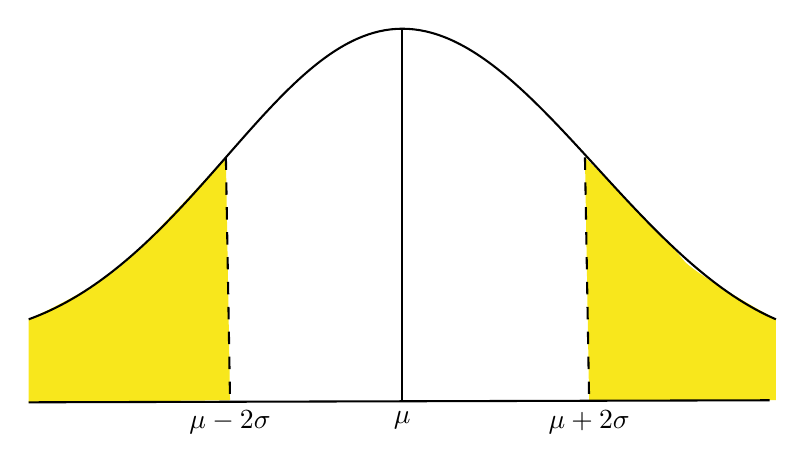
\begin{tikzpicture}[x=0.75pt,y=0.75pt,yscale=-1,xscale=1]
        %uncomment if require: \path (0,300); %set diagram left start at 0, and has height of 300
        
        %Shape: Polygon Curved [id:ds4299421394348286] 
        \draw  [draw opacity=0][fill={rgb, 255:red, 248; green, 231; blue, 28 }  ,fill opacity=1 ] (70,200) .. controls (70,200) and (103,185) .. (116,173) .. controls (129,161) and (165,122) .. (165,122) .. controls (165,122) and (167,239) .. (167,239) .. controls (167,239) and (70,240) .. (70,240) .. controls (70,240) and (70,200) .. (70,200) -- cycle ;
        %Shape: Polygon Curved [id:ds342419034869045] 
        \draw  [draw opacity=0][fill={rgb, 255:red, 248; green, 231; blue, 28 }  ,fill opacity=1 ] (338,122) .. controls (338,122) and (380,164) .. (385,171) .. controls (390,178) and (430,200) .. (430,200) .. controls (430,200) and (430,239) .. (430,239) .. controls (430,239) and (340,239) .. (340,239) .. controls (340,239) and (338,122) .. (338,122) -- cycle ;
        %Straight Lines [id:da18625365603208555] 
        \draw    (70,240) -- (427,239.01) ;
        %Straight Lines [id:da37636810464348036] 
        \draw  [dash pattern={on 4.5pt off 4.5pt}]  (338,122) -- (340,239) ;
        %Curve Lines [id:da1940644130383995] 
        \draw    (70,200) .. controls (150,171) and (190,60) .. (250,60) .. controls (310,60) and (360,170) .. (430,200) ;
        %Straight Lines [id:da3467386125082421] 
        \draw  [dash pattern={on 4.5pt off 4.5pt}]  (165,122) -- (167,239) ;
        %Straight Lines [id:da41423441599411515] 
        \draw    (250,60) -- (250,239.5) ;
        
        % Text Node
        \draw (340,242.4) node [anchor=north] [inner sep=0.75pt]    {$\mu +2\sigma $};
        % Text Node
        \draw (167,242.4) node [anchor=north] [inner sep=0.75pt]    {$\mu -2\sigma $};

        % Text Node
        \draw (250,242.9) node [anchor=north] [inner sep=0.75pt]    {$\mu $};
    \end{tikzpicture}
\end{example} 

\begin{definition}[Median]
    Suppose that $X$ is a continuous RV, the \vocab{median} of $X$ is the number $m$ s.t.
    \[\mathbb{P}(X\leq m) = \mathbb{P}(X\geq m) = \frac{1}{2}\]
    In other words
    \[\int_{-\infty}^mf(x)\,\,d x = \int_0^{\infty}f(x)\,\,d x = \frac{1}{2}\]
\end{definition}

\begin{remark} ~
    \begin{itemize}
        \item For $X \sim \mathcal{N}(\mu, \sigma^2)$ and other distributions symmetric about their mean, the median $m = \mathbb{E}[X]$.
        \item \color{blue} Sometimes $|X - m|$ better than $|X - \mu|$ for interpretation. \color{black}
    \end{itemize} 
\end{remark} 

\subsection{More than one continuous RVs}
Allow RVs to take values in $\mathbb{R}^n$. \\ 
E.g. $X = (X_1,\dots,X_n) \in \R^n$ a RV. \\

\begin{definition}[Multivarite Density Function]
    We say that $X$ has \vocab{multivariate density} $f : \mathbb{R} \to [0, \infty)$ if
    \begin{align*}
        \mathbb{P}(X_1\leq x_1,\dots,X_n\leq x_n) &= \underbracket{\int_{-\infty}^{x_1}\dots \int_{-\infty}^{x_n}}_{\color{red} \text{Integrate over } (- \infty, x_1] \times \dots \times (-\infty, x_n]} f(u_1,\dots,u_n) \underbracket{\prod du_i}_{\color{red} \text{i.e. } \,du_1 \dots \,du_n} \\
        &= \int_{-\infty}^{x_1}\dots \int_{-\infty}^{x_n} f(u_1,\dots,u_n) \prod du_i.
    \end{align*} 
    $f$ is sometimes also called (especially for $n = 2$) a joint density function.
\end{definition} 

\underline{Consequence}: This generalises: $\mathbb{P}\left( (X_1, \dots, X_n) \in A \right) = \int_A f(\bm{u}) \,d \bm{u}$ for all \color{red} ``measurable'' \color{black} $A \in \mathbb{R}^n$.

\begin{definition}[Independence]
    We say that $X_1,\dots,X_n$ are \vocab{independent} if $\forall x_1,\dots,x_n$,
    \[\mathbb{P}(X_1\leq x_1,\dots,X_n\leq x_n) = \mathbb{P}(X_1\leq x_1)\dots \mathbb{P}(X_n\leq x_n)\]
\end{definition}

Goal: convert to statement about densities

\begin{definition}[Marginal Density]
    Let $X = (X_1, \dots, X_n)$ have density $f$.
    The \vocab{marginal density} $f_{X_i}$ of $X_i$ is 
    \begin{align*}
        f_{X_i}(x_i) &= \int_{-\infty}^{\infty} \dots \int_{-\infty}^{\infty} f(x_1, \dots, x_n) \prod_{\color{red} j \neq i} dx_j
    \end{align*} 
    \color{blue} ``The density of $X_i$ viewed as a RV by itself. We fix $x_i$ and let everything else vary.''
\end{definition} 

\begin{theorem}
    Let $X = (X_1,\dots,X_n)$ has density $f$.
    \begin{enumerate}
        \item If $X_1,\dots,X_n$ are independent with marginals $f_{X_1},\dots, f_{X_n}$. Then $f(x_1, \dots, x_n) = f_{X_1}(x_1) \dots f_{X_n}(x_n)$
        \item Suppose that $f$ factorises as $f(x_1, \dots, x_n) = g_1(x_1) \dots g_n(x_n)$ for some non-negative functions $(g_i)$. Then $X_1,\dots, X_n$ are independent and marginal $f_{X_i} \propto g_i$.
    \end{enumerate}
\end{theorem}

\begin{proof} ~
    \begin{enumerate}
        \mathitem \begin{align*}
            \mathbb{P}(X_1\leq x_1,\dots, X_n\leq x_n) &= \mathbb{P}(X_1\leq x_1)\dots \mathbb{P}(X_n\leq x_n)\\
            &= \left[ \int_{-\infty}^{x_1} f_{X_1}(u_1) \,du_1 \right] \dots \left[ \int_{-\infty}^{x_n} f_{X_n}(u_n) \,du_n \right] \\
            &=\int_{-\infty}^{x_1} \dots \int_{-\infty}^{x_n} \underbracket{\prod f_{X_i}(u_i)}_{\color{red} \text{matches definition of } f} \prod du_i
        \end{align*}
        \item \underline{Idea}: \begin{itemize}
            \item replace $g_i(x)$ with $h_i(x) = \frac{g_i(x)}{\int g_i(u) \,du}$ so $h_i$ \emph{is} a density.
            \item compute integrals for $\mathbb{P}(X_1\leq x_1,\dots,X_n\leq x_n)$ and $\mathbb{P}(X_1\leq x_1)\dots \mathbb{P}(X_n\leq x_n)$ and show equality.
        \end{itemize} 
    \end{enumerate}
\end{proof}

\subsection{Transformation of Multiple RVs}

\begin{example}
    Let $X$ and $Y$ be independent RVs with densities $f_X$ and $f_Y$ respectively. \\
    \underline{Goal}: density of $Z = X + Y$.
    \begin{align*}
        \mathbb{P}(X + Y \leq z) &= \underset{\{x+y\leq z\}}{\int\int} f_{X,Y}(x,y) \,dx \,dy \\
        &= \int_{x=-\infty}^{\infty} \int_{y = -\infty}^{z-x} f_X(x)f_Y(y) \,dx \,dy
        \intertext{Substitute $y' = y + x$}
        &=\int_{x = -\infty}^{\infty} \left(\int_{y' = -\infty}^z f_X(x) f_Y(y'-x) \,d y' \right) \,d x \\
        \intertext{$y' \mapsto y$}
        &=\int_{y = -\infty}^z \,d y \left(\int_{x = -\infty}^{\infty} f_X(x) f_Y(y-x) \,d x\right)
        \intertext{So the density of $Z$ is:}
        f_Z(z) &= \int_{-\infty}^{\infty} f_Y(z - x) f_X(x) \,d x
    \end{align*}
    We call this function the \emph{convolution} of $f_X$ and $f_Y$.

    \color{blue}
    For $X, Y$ discrete, non-negative and independent we would have \begin{align*}
        \mathbb{P}(X + Y = k) = \sum_{l = 0}^{k} \mathbb{P}(X = \ell) \mathbb{P}(Y = k - \ell)
    \end{align*} 
\end{example} 

\begin{definition}[Gamma Distribution]
    The \vocab{gamma distribution} has two parameters $\lambda > 0$ and $n \in \mathbb{N}$.
    Its range is $[0, \infty)$.
    We say $X \sim \Gamma(n, \lambda)$ and has density
    \begin{align*}
        f_X(x) &= e^{-\lambda x} x^{n - 1} \frac{\lambda^n}{(n - 1)!} \\
        n = 1 &\mapsto \operatorname{Exp}(\lambda) \\
        n = 2 &\mapsto \lambda^2 x e^{-\lambda x}
    \end{align*} 
\end{definition} 

\begin{example}[Exponential Distribution]
    Let $X, Y \sim \operatorname{Exp}(\lambda)$ be IID and $Z = X + Y$.
    \begin{align*}
        f_Z(z) &= \int_{-\infty}^{\infty} \lambda e^{-\lambda (z - x)} \lambda e^{-\lambda x} \,dx \\
        &= \int_{0}^{z} \lambda^2 e^{-\lambda z} \,dx \\
        &= \lambda^2 z e^{-\lambda z}.
    \end{align*} 
    So $X + Y \sim \Gamma(2, \lambda)$ and in fact the sum of $n$ IID $\operatorname{Exp}(\lambda)$ has distribution $\Gamma(n, \lambda)$.
\end{example} 

\begin{example}[Normal Distribution] \label{exm:transnormal}
    Let $X_1 \sim \mathcal{N}(\mu_1, \sigma_1^2), X_2 \sim \mathcal{N}(\mu_2, \sigma_2^2)$ be independent. \\
    Then $X_1 + X_2 \sim \color{red}\mathcal{N}\color{black} (\mu_1, + \mu_2, \sigma_1^2 + \sigma_2^2)$ (We already know what the mean and variance of $X_1 + X_2$ is, the interesting part is that it is normal). \\
    We can prove this using convolution but we will prove it using generating functions soon, \Cref{exm:mgf-normal}.
\end{example} 

\begin{theorem}
    Let $X = (X_1, \dots, X_n)$ be a RV on $D \in \mathbb{R}^n$, $g : \mathbb{R}^n \to \mathbb{R}^n$ a well-behaved and $U = g(X) = (U_1, \dots, U_n)$.
    Assume the joint density $f_X(x)$ is continuous. \\
    Then the joint density \begin{align*}
        f_U(\bm{u}) &= f_X \left( g^{-1} (\bm{u}) \right) | J(\bm{u}) | 
        \intertext{where $J$, the Jacobean, is}
        J &= \det \left( \underbracket{\left( \frac{\partial [g^{-1}(\bm{u})]_i }{\partial u_j} \right)^n_{i, j = 1}}_{n \times n \text{ matrix}} \right)
    \end{align*} 
\end{theorem} 

\begin{proof}[``Proof'']
    Definition of multivariate integration by substitution.
\end{proof} 

\color{red} \underline{Top tip}: $| \text{Jacobean of } g^{-1}| = \frac{1}{| \text{Jacobean of } g|}$. \color{black}

\begin{example}[Radial symmetry]
    Let $X, Y \sim \mathcal{N}(0, 1)$ be IID. \\
    Let $(X, Y) = \underbracket{(R \cos \Theta, R \sin \Theta)}_{\color{red} g^{-1}}$. \\
    \underline{Range}: $R > 0, \Theta \in [0, 2 \pi)$.
    
    \tikzset{every picture/.style={line width=0.75pt}} %set default line width to 0.75pt        
    
    \begin{tikzpicture}[x=0.75pt,y=0.75pt,yscale=-1,xscale=1]
    %uncomment if require: \path (0,300); %set diagram left start at 0, and has height of 300
    
    %Straight Lines [id:da10390451102215748] 
    \draw    (90,170) -- (303.99,169.41) -- (447,169.01) ;
    \draw [shift={(450,169)}, rotate = 539.8399999999999] [fill={rgb, 255:red, 0; green, 0; blue, 0 }  ][line width=0.08]  [draw opacity=0] (8.93,-4.29) -- (0,0) -- (8.93,4.29) -- cycle    ;
    %Straight Lines [id:da2629289175779972] 
    \draw    (260,250) -- (260,64) ;
    \draw [shift={(260,61)}, rotate = 450] [fill={rgb, 255:red, 0; green, 0; blue, 0 }  ][line width=0.08]  [draw opacity=0] (8.93,-4.29) -- (0,0) -- (8.93,4.29) -- cycle    ;
    %Straight Lines [id:da30035531926850356] 
    \draw    (320,100) -- (260,170) ;
    %Shape: Circle [id:dp24427218103249926] 
    \draw  [color={rgb, 255:red, 0; green, 0; blue, 0 }  ,draw opacity=1 ][fill={rgb, 255:red, 0; green, 0; blue, 0 }  ,fill opacity=1 ] (315,100) .. controls (315,97.24) and (317.24,95) .. (320,95) .. controls (322.76,95) and (325,97.24) .. (325,100) .. controls (325,102.76) and (322.76,105) .. (320,105) .. controls (317.24,105) and (315,102.76) .. (315,100) -- cycle ;
    %Shape: Arc [id:dp03489733067827139] 
    \draw  [draw opacity=0] (272.62,154.49) .. controls (276.94,158) and (279.76,163.29) .. (279.99,169.23) -- (260,170) -- cycle ; \draw   (272.62,154.49) .. controls (276.94,158) and (279.76,163.29) .. (279.99,169.23) ;
    
    % Text Node
    \draw (322,96.6) node [anchor=south west] [inner sep=0.75pt]    {$( X,Y)$};
    % Text Node
    \draw (293,160) node    {$\theta $};
    
    
    \end{tikzpicture}

    \begin{align*}
        f_{X, Y}(x, y) &= \frac{1}{\sqrt{2 \pi}} e^{-\frac{x^2}{2}} \frac{1}{\sqrt{2 \pi}} e^{-\frac{y^2}{2}} \\
        &= \frac{1}{2 \pi} e^{-\frac{x^2 + y^2}{2}} \\
        J &= \begin{vmatrix} \cos \theta & - r \sin \theta \\ \sin \theta & r \cos \theta \end{vmatrix} \\
        &= r. \\
        \implies f_{R, \Theta}(r,\theta) &= \color{blue} \frac{1}{2\pi} \color{red} e^{- \frac{r^2}{2}} \times r \\
        f_\Theta(\theta) &= \frac{1}{2 \pi} \\
        f_R(r) &= e^{- \frac{r^2}{2}} r
    \end{align*} 
    Thus $\Theta, R$ are independent and $\Theta$ is uniform on $[0, 2 \pi)$.    
\end{example}

\underline{Warning}: Change of range. \\
Eg: $X, Y \geq 0$. $Z = X + Y$.
\begin{align*}
    f_{X, Z}(x, z) &= \color{red}?\color{black} (x, z) 1_{z \geq x}
\end{align*} so $X, Z$ are \emph{not} independent even if $\color{red}?\color{black}$ splits as a product.

% Pattern Info
 
\tikzset{
pattern size/.store in=\mcSize, 
pattern size = 5pt,
pattern thickness/.store in=\mcThickness, 
pattern thickness = 0.3pt,
pattern radius/.store in=\mcRadius, 
pattern radius = 1pt}
\makeatletter
\pgfutil@ifundefined{pgf@pattern@name@_kl8aonlcq}{
\pgfdeclarepatternformonly[\mcThickness,\mcSize]{_kl8aonlcq}
{\pgfqpoint{0pt}{-\mcThickness}}
{\pgfpoint{\mcSize}{\mcSize}}
{\pgfpoint{\mcSize}{\mcSize}}
{
\pgfsetcolor{\tikz@pattern@color}
\pgfsetlinewidth{\mcThickness}
\pgfpathmoveto{\pgfqpoint{0pt}{\mcSize}}
\pgfpathlineto{\pgfpoint{\mcSize+\mcThickness}{-\mcThickness}}
\pgfusepath{stroke}
}}
\makeatother

% Pattern Info
 
\tikzset{
pattern size/.store in=\mcSize, 
pattern size = 5pt,
pattern thickness/.store in=\mcThickness, 
pattern thickness = 0.3pt,
pattern radius/.store in=\mcRadius, 
pattern radius = 1pt}
\makeatletter
\pgfutil@ifundefined{pgf@pattern@name@_tbwhexxct}{
\pgfdeclarepatternformonly[\mcThickness,\mcSize]{_tbwhexxct}
{\pgfqpoint{0pt}{-\mcThickness}}
{\pgfpoint{\mcSize}{\mcSize}}
{\pgfpoint{\mcSize}{\mcSize}}
{
\pgfsetcolor{\tikz@pattern@color}
\pgfsetlinewidth{\mcThickness}
\pgfpathmoveto{\pgfqpoint{0pt}{\mcSize}}
\pgfpathlineto{\pgfpoint{\mcSize+\mcThickness}{-\mcThickness}}
\pgfusepath{stroke}
}}
\makeatother
\tikzset{every picture/.style={line width=0.75pt}} %set default line width to 0.75pt        

\begin{tikzpicture}[x=0.75pt,y=0.75pt,yscale=-1,xscale=1]
%uncomment if require: \path (0,300); %set diagram left start at 0, and has height of 300

%Straight Lines [id:da03274320383110729] 
\draw [color={rgb, 255:red, 126; green, 211; blue, 33 }  ,draw opacity=1 ]   (554.36,62.45) -- (384.22,222.8) ;
%Shape: Right Triangle [id:dp5442274211530183] 
\draw  [draw opacity=0][pattern=_kl8aonlcq,pattern size=15pt,pattern thickness=0.75pt,pattern radius=0pt, pattern color={rgb, 255:red, 126; green, 211; blue, 33}] (554.36,62.45) -- (384.22,222.8) -- (384.22,62.45) -- cycle ;
%Shape: Rectangle [id:dp7490728127335207] 
\draw  [color={rgb, 255:red, 255; green, 255; blue, 255 }  ,draw opacity=0 ][pattern=_tbwhexxct,pattern size=15pt,pattern thickness=0.75pt,pattern radius=0pt, pattern color={rgb, 255:red, 126; green, 211; blue, 33}] (69.04,58.95) -- (239.18,58.95) -- (239.18,219.3) -- (69.04,219.3) -- cycle ;
%Shape: Axis 2D [id:dp7641223820654799] 
\draw  (50,219.3) -- (240.36,219.3)(69.04,60) -- (69.04,237) (233.36,214.3) -- (240.36,219.3) -- (233.36,224.3) (64.04,67) -- (69.04,60) -- (74.04,67)  ;
%Shape: Axis 2D [id:dp49924282326387726] 
\draw  (365.18,222.8) -- (555.55,222.8)(384.22,63.5) -- (384.22,240.5) (548.55,217.8) -- (555.55,222.8) -- (548.55,227.8) (379.22,70.5) -- (384.22,63.5) -- (389.22,70.5)  ;

% Text Node
\draw (49,55.4) node [anchor=north west][inner sep=0.75pt]    {$Y$};
% Text Node
\draw (230.5,226.9) node [anchor=north west][inner sep=0.75pt]    {$X$};
% Text Node
\draw (364.18,58.9) node [anchor=north west][inner sep=0.75pt]    {$Z$};
% Text Node
\draw (545.68,230.4) node [anchor=north west][inner sep=0.75pt]    {$X$};


\end{tikzpicture}

\subsection{Moment Generating Function}

\begin{definition}[Moment Generating Function]
    Let $X$ have density $f$.
    The \vocab{MGF} of $X$ is 
    \begin{align*}
        m_X(\theta) &= \mathbb{E}[e^{\theta X}] \\
        &= \int_{-\infty}^{\infty} e^{\theta x} f(x) \,dx
    \end{align*} whenever this is finite.
\end{definition} 

\begin{note}
    $m_X(0) = 1$.
\end{note} 

\begin{theorem}
    The MGF uniquely determines distribution of a RV whenever it exists $\forall \; \theta \in (- \epsilon, \epsilon)$ for some $\epsilon > 0$.
\end{theorem} 

\begin{definition}[Moment]
    The $n$th moment of $X$ is $\mathbb{E}[X^n]$.
\end{definition} 

\begin{theorem}
    Suppose $m(\theta)$ exists $\forall \; \theta \in (- \epsilon, \epsilon)$.
    Then $m^{(n)}(0) = \left. \frac{d^n}{d \theta^n} m(\theta) \right|_{m = 0} = \mathbb{E}[X^n]$.
\end{theorem} 

\color{blue}
\underline{Proof comment}: Use $\frac{\partial^n e^{\theta x}}{\partial \theta^n} = x^n e^{\theta x}$.
\color{black}

\begin{claim}
    Let $X_1, \dots, X_n$ be independent and $X = X_1 + \dots + X_n$.
    Then \begin{align*}
        m_X(\theta) &= \mathbb{E}[e^{\theta (X_1 + \dots + X_n)}] \\
        &= \mathbb{E}[e^{\theta X_1}] \dots \mathbb{E}[e^{\theta X_n}] \ \text{ by independence} \\
        &= \prod m_{X_i}(\theta).
    \end{align*} 
\end{claim} 

\begin{example}[Gamma Distribution]
    Let $X \sim \Gamma(n, \lambda)$.
    \begin{align*}
        f_X(x) &= e^{-\lambda x} \frac{\lambda^n x^{n - 1}}{(n - 1)!} \\
        m(\theta) &= \int_{0}^{\infty} e^{\theta x} e^{-\lambda x} \frac{\lambda^n x^{n - 1}}{(n - 1)!} \,dx 
        \intertext{Goal: Reduce to integral of pdf over range!}
        &= \int_{0}^{\infty} e^{-(\lambda - \theta)x} x^{n - 1} \times \frac{\lambda^n}{(n - 1)!} \,dx \\
        &= \left( \frac{\lambda}{\lambda - \theta} \right)^n \int_{0}^{\infty} \underbracket{e^{-(\lambda - \theta)} x^{n - 1} \frac{(\lambda - \theta)^n}{(n - 1)!}}_{\text{pdf of } \operatorname{\Gamma}(n, \lambda - \theta)\footnote{provided $\theta < \lambda$.}} \,dx \\
        &= \begin{cases}
            \left( \frac{\lambda}{\lambda - \theta} \right)^n & \theta < \lambda \\
            \infty & \theta \geq \lambda.
        \end{cases} 
    \end{align*} 
    So $\operatorname{Exp}(\lambda)$ has MGF $\frac{\lambda}{\lambda - \theta}$.
    And we've proved that the sum of $n$ IID $\operatorname{Exp}(\lambda)$ has distribution $\Gamma(n, \lambda)$.
\end{example} 

\begin{example}[Normal Distribution] \label{exm:mgf-normal}
    Let $X \sim \mathcal{N}(\mu, \sigma^2)$.
    \begin{align*}
        f_X(x) &= \frac{1}{\sqrt{2 \pi \sigma^2}} \exp \left( - \frac{(x - \mu)^2}{2 \sigma^2} \right) \\
        m_X(\theta) &= \exp \left( \theta \mu + \frac{\theta^2 \sigma^2}{2} \right)
    \end{align*}
    The proof is left as an exercise, try relating integral to integral of pdf of some normal distribution. \\
    Let $X_1 \sim \mathcal{N}(\mu_1, \sigma_1^2)$, $X_2 \sim \mathcal{N}(\mu_2, \sigma_2^2)$ be independent.
    Then 
    \begin{align*}
        m_{X_1 + X_2}(\theta) &= \exp \left(\theta \mu_1 + \frac{\theta^2 \sigma_1^2}{2} \right) \exp \left( \theta \mu_2 + \frac{\theta^2 \sigma_2^2}{2} \right) \\
        &= \underbracket{\exp \left( \theta (\mu_1 + \mu_2) + \frac{\theta^2}{2} (\sigma_1^2 + \sigma_2^2) \right)}_{\text{MGF of } \mathcal{N}(\mu_1 + \mu_2, \sigma_1^2 + \sigma_2^2)}
    \end{align*}
\end{example}

\subsection{Convergence of RVs}

\begin{definition}[Convergence in Distribution]
    Let $(X_n)_{n \geq 1}$ and $X$ be RVs.
    $X_n$ \underline{converges to} $X$ \underline{in distribution}, $X_n \overset{d}{\to} X$, if $F_{X_n}(x) \to F_X(x)$ for all $x \in \mathbb{R}$ which are continuity points of $F_X$.
\end{definition} 

\begin{example} \label{exm:conv1}
    Let $X_n = \frac{1}{n} \operatorname{Unif}\left( {1, \dots, n} \right)$ and $X \sim \operatorname{Unif} [0, 1]$.
    {\par \centering 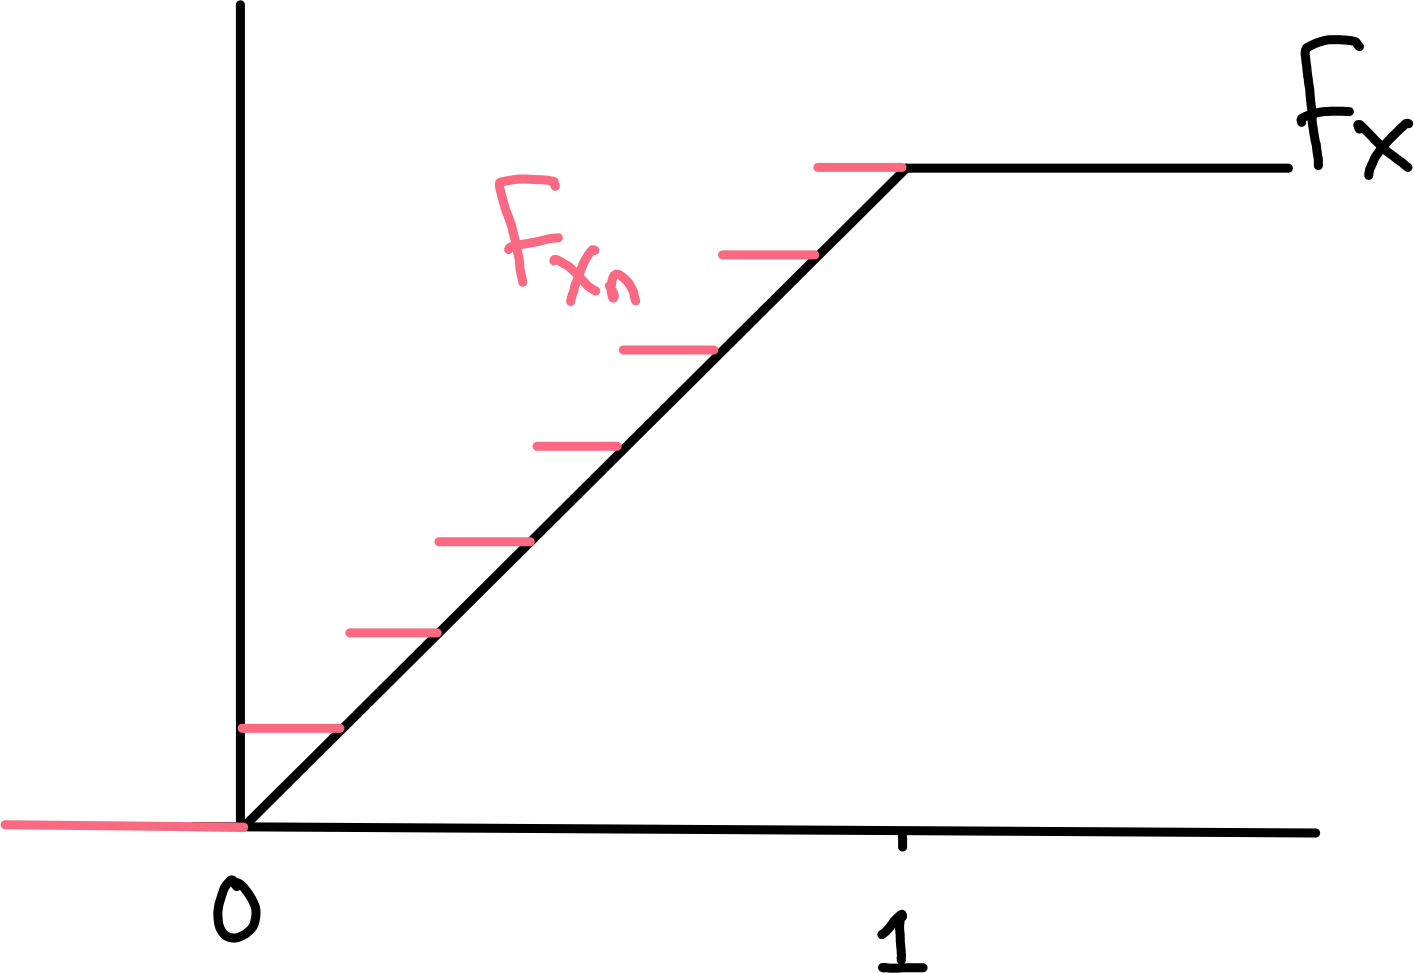
\includegraphics[height=5cm]{05-discuniform} \par}
    $F_X$ continuous, $F_{X_n} \to F_X(x)$ holds $\forall \; x \in [0, 1]$ by picture so $X_n \overset{d}{\to} X$.
\end{example} 

\begin{example} ~\vspace*{-1.5\baselineskip}
    \begin{align*}
        X_n &= \begin{cases}
            0 & \mathbb{P} = \frac{1}{2} \\
            1 + \frac{1}{n} & \mathbb{P} = \frac{1}{2}
        \end{cases} \\
        F_{X_n}(x) &= \begin{cases}
            \frac{1}{2} & x \in (0, 1) \\
            \frac{1}{2} & x = 1 \\
            1 & x > 1 \text{ when $n$ is large}
        \end{cases} \\
        \text{Let } X &\sim \operatorname{Bern}\left( \frac{1}{2} \right) \\
        F_X(1) &= 1.
    \end{align*} 
    But $F_X$ has a discontinuity at $x = 1$ so $X_n \overset{d}{\to} X$.
    {\par \centering 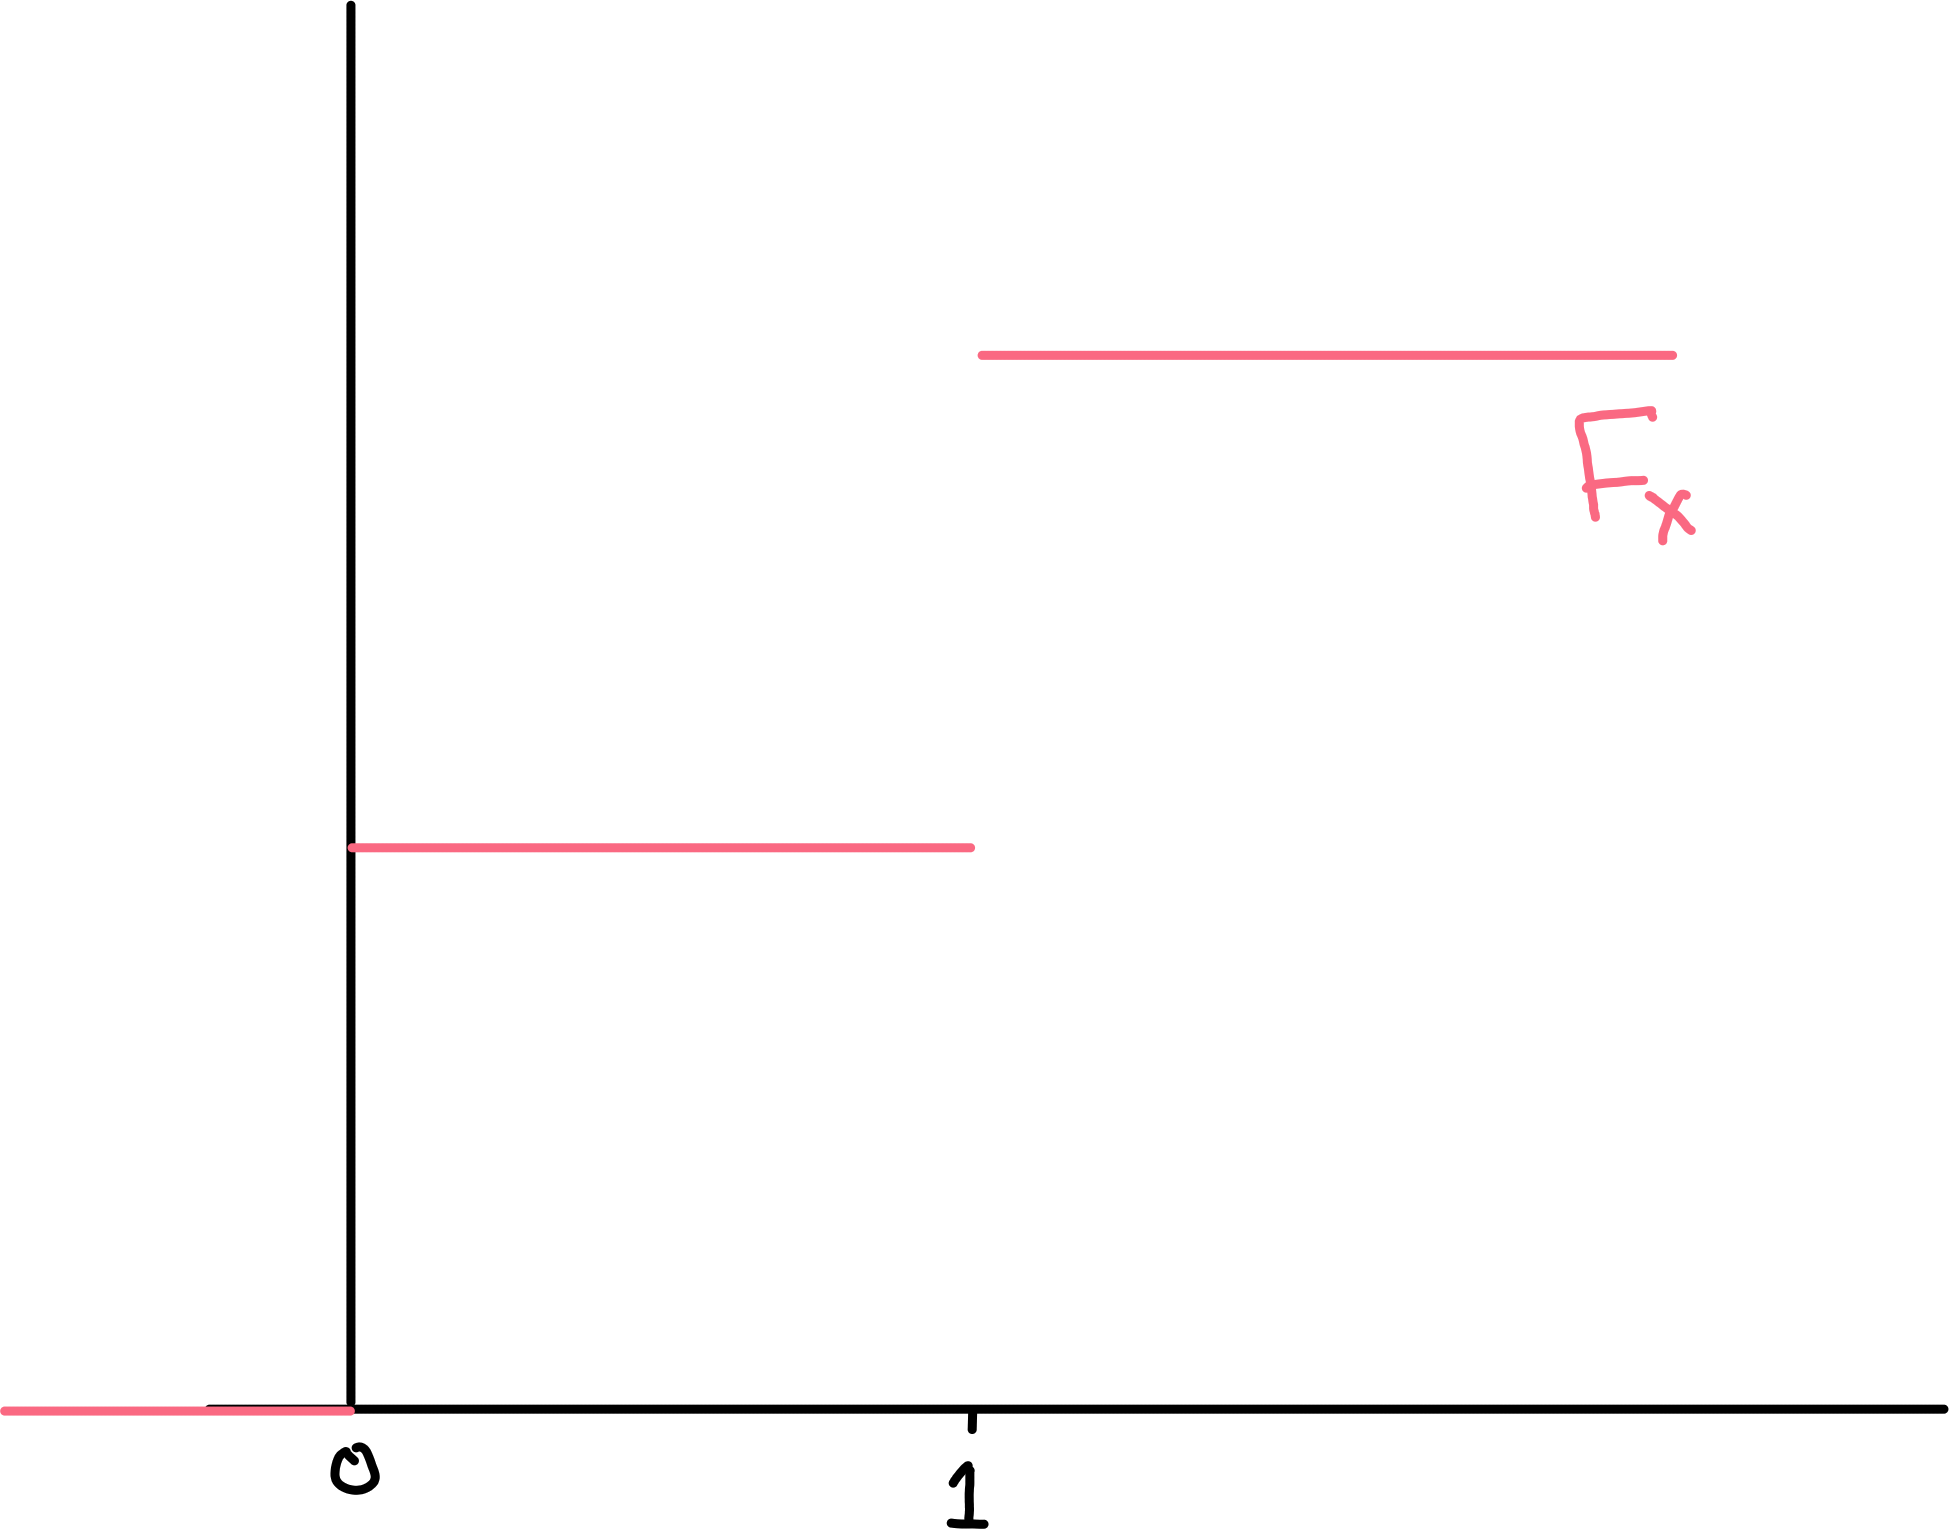
\includegraphics[height=5cm]{05-discbern} \par}
    (I.e. deterministic convergence of a sequence of real numbers is an example of convergence in distribution)
\end{example} 

\begin{claim}
    If $X$ is a constant $c$, then convergence in distribution is equivalent to: $\forall \; \epsilon > 0: \ \mathbb{P}(|X_n - c| > \epsilon) \to 0$ as $n \to \infty$. \color{blue} ``convergence in probability to constant''.
\end{claim} 

\begin{claim}
    If $X$ is a continuous RV with $X_n \overset{d}{\to} X$ then $\mathbb{P}(a \leq X_n \leq b) \to \mathbb{P}(a \leq X \leq b)$ for all $a, b \in [-\infty, \infty]$.
\end{claim} 

Warning: Does not say that \underline{densities} converge, e.g. in \Cref{exm:conv1}, $X_n$ does not have a density.

\subsection{Laws of Large Numbers}

\begin{align*}
    \frac{S_n}{n} ``\to" \mu
\end{align*} 

\begin{theorem}[Weak LLN]
    Let $(X_n)_{n \geq 1}$ be IID with $\mu = \mathbb{E}[X_1]$ finite. 
    Set $S_n = X_1 + \dots + X_n \quad \forall \; n \geq 0$.
    Then
    \begin{align*}
        \forall \; \epsilon > 0: \ \mathbb{P}\left( \left|\frac{S_n}{n} - \mu \right| > \epsilon \right) \to 0 \text{ as } n \to \infty
    \end{align*} 
\end{theorem} 

\begin{proof}
    (Assume $\Var(X_1) = \sigma^2 < \infty$)
    \begin{align*}
        \mathbb{P}\left( \left|\frac{S_n}{n} - \mu\footnote{\color{red} Also $\mathbb{E}\left[\frac{S_n}{n}\right]$} \right| > \epsilon \right) &= \mathbb{P}\left( \left| S_n - n \mu \right| > \epsilon n \right) \\
        &\leq \frac{\Var(S_n)}{\epsilon^2 n^2} \ \text{ by \nameref{prp:cheby}} \\
        &= \frac{n \sigma^2}{\epsilon^2 n^2} \to 0 \ \text{ as } n \to \infty.
    \end{align*}
    $\epsilon > 0$ is fixed we are not taking limit as $\epsilon \to 0$.
\end{proof} 

\subsection{Central Limit Theorem}

\begin{theorem}[Central Limit Theorem]
    Let $(X_n)_{n \geq 1}$ be IID with $\mu = \mathbb{E}[X_1]$ finite \color{red} and $\sigma^2 < \infty$\color{black}. 
    Set $S_n = X_1 + \dots + X_n \quad \forall \; n \geq 0$.
    Then
    \begin{align*}
        \frac{S_n - n \mu}{\sqrt{n \sigma^2}} \overset{d}{\to} \mathcal{N}(0, 1) \text{ as } n \to \infty.
    \end{align*} 
\end{theorem} 

\underline{Discussion}: Three stage summary
\begin{enumerate}
    \item Distribution of $S_n$ concentrated on $n \mu$ - we already know this from WLLN.
    \item \color{red} Fluctuations around $n \mu$ have order $\sqrt{n}$ - new and important \color{black}
    \item Shape is normal - detail.
\end{enumerate} 

We use CLT by 
\begin{enumerate}
    \item $S_n \overset{d}{\approx} \mathcal{N}(n \mu, n \sigma^2)$
    \mathitem 
    \begin{align*}
        \mathbb{P}(a \leq S_n \leq b) &= \mathbb{P}\left( \frac{a - n \mu}{\sqrt{n \sigma^2}} \leq \frac{S_n - n \mu}{\sqrt{n \sigma^2}} \leq \frac{b - n \mu}{\sqrt{n \sigma^2}} \right). \\
        &= \mathbb{P} \left( \frac{a - n \mu}{\sqrt{n \sigma^2}} \leq Z \leq \frac{b - n \mu}{\sqrt{n \sigma^2}} \right).
    \end{align*} 
\end{enumerate} 

\begin{theorem}[Continuity Theorem for MGFs]
    Let $(X_n)$ and $X$ have MGFs $m_{X_n}$ and $m_X$.
    If \begin{itemize}
        \item $m_X(\theta) < \infty$ for $\theta \in (-\epsilon, \epsilon)$.
        \item $m_{X_n}(\theta) \to m_X(\theta) \quad \forall \; \theta \text{ s.t. } m_X(\theta) < \infty$.
    \end{itemize} 
    Then $X_n \overset{d}{\to} X$.
\end{theorem} 

\begin{proof}
    Part II Probability and Measure.
\end{proof} 

\underline{Idea}: Expand $m_X(\theta)$ as a Taylor series around $0$.
\begin{align*}
    m_X(\theta) &= 1 + m_X'(0) \theta + \frac{m_X''(0)}{2!} \theta^2 + \dots \\
    &= 1 + \theta \mathbb{E}[X] + \frac{1}{2} \theta^2 \mathbb{E}[X^2] + o(\theta^2)
\end{align*} 

\begin{proof}[Proof - WLLN via MGFs] ~

    Comment: We know MGF of $S_n$, we want to study the MGF of $S_n / n$.
    \begin{align*}
        m_{S_n / n}(\theta) &= \mathbb{E}\left[\exp \left( \theta \frac{S_n}{n} \right) \right] \\
        &= \mathbb{E}\left[\exp \left( \frac{\theta}{n} S_n \right) \right] \ \text{\color{red} Key step}. \\
        &= m_{S_n}(\theta / n) \\
        &= m_{X_1}(\theta / n) \dots m_{X_n}(\theta / n) \\
        &= \left( 1 + \mu \frac{\theta}{n} + o \left( \frac{1}{n} \right) \right)^n \\
        &\to e^{\mu \theta}
    \end{align*} 
    $e^{\mu \theta}$ is the MGF of the RV $X = \mu$ with $\mathbb{P} = 1$, so $\frac{S_n}{n} \overset{d}{\to} \mu$ by the continuity theorem.
\end{proof} 

\begin{proof}[Proof - CLT via MGFs] ~

    Assume WLOG $\mu = 0$ and $\sigma^2 = 1$. (so $\mathbb{E}[X_i^2] = 1$). 
    In general $X \mapsto \frac{X - \mu}{\sqrt{\sigma^2}}$

    STP: $S_n / \sqrt{n} \overset{d}{\to} \mathcal{N}(0, 1)$.
    \begin{align*}
        m_{X_i}(\theta) &= 1 + \frac{\theta^2}{2} + o(\theta^2) \\
        m_{S_n / \sqrt{n}}(\theta) &= \mathbb{E}\left[\exp \left( \theta \frac{S_n}{\sqrt{n}} \right) \right] \\
        &= \mathbb{E}\left[\exp \left( \frac{\theta}{\sqrt{n}} S_n \right) \right] \\
        &= m_{S_n}(\theta / \sqrt{n}) \\
        &= m_{X_1}(\theta / \sqrt{n}) \dots m_{X_n}(\theta / \sqrt{n}) \\
        &= \left( 1 +  \frac{\theta^2}{2n} + o \left( \frac{1}{n} \right) \right)^n \\
        &\to e^{\theta^2 / 2}
    \end{align*} 
    $e^{\theta^2 / 2}$ is the MGF of the $\mathcal{N}(0, 1)$.
\end{proof} 

\begin{theorem}[Strong LLN]
    Let $(X_n)_{n \geq 1}$ be IID with $\mu = \mathbb{E}[X_1]$ finite and $\sigma^2 < \infty$. 
    Set $S_n = X_1 + \dots + X_n \quad \forall \; n \geq 0$.
    Then
    \begin{align*}
        \mathbb{P}\left( \frac{S_n}{n} \to \mu \text{ as } n \to \infty \right) = 1.
    \end{align*} 
    \color{blue} ``almost sure convergence'' or ``convergence with probability 1''.
\end{theorem} 

\subsection{Inequalities for $\mathbb{E}[f(X)]$}
\underline{Motivation}: For $f(x) = x^2$ we know $\mathbb{E}[f(X)] \geq f(\mathbb{E}[X])$ as $\Var(X) \geq 0$.

\begin{question}
    What about general $f$?
\end{question} 

\begin{definition}[Convex Function]
    A function $f: \mathbb{R} \to \mathbb{R}$ is \vocab{convex} if $\forall \; x, y \in \mathbb{R}$ and $t \in [0, 1]$ \begin{align*}
        f \left( tx + (1 - t)y \right) \leq t f(x) + (1 - t) f(y).
    \end{align*}
    
    \tikzset{every picture/.style={line width=0.75pt}} %set default line width to 0.75pt        

    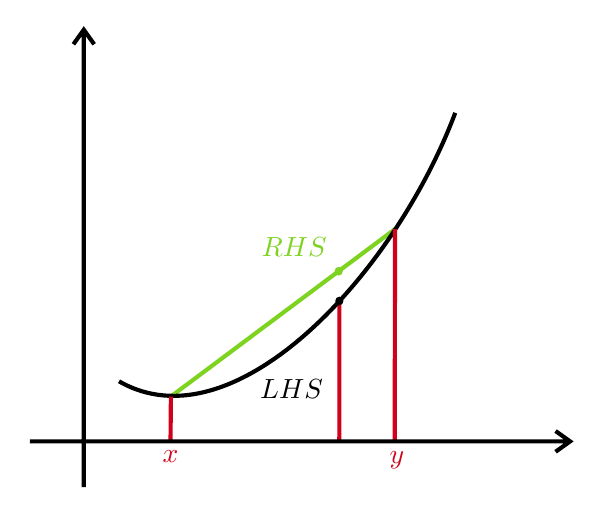
\begin{tikzpicture}[x=0.75pt,y=0.75pt,yscale=-1,xscale=1]
    %uncomment if require: \path (0,300); %set diagram left start at 0, and has height of 300

    %Straight Lines [id:da4293917761962731] 
    \draw [color={rgb, 255:red, 208; green, 2; blue, 27 }  ,draw opacity=1 ][line width=1.5]    (198.5,182.01) -- (198.48,249.59) ;
    %Straight Lines [id:da6814245690866725] 
    \draw [color={rgb, 255:red, 126; green, 211; blue, 33 }  ,draw opacity=1 ][line width=1.5]    (117.33,228.03) -- (225.33,147.36) ;
    %Curve Lines [id:da6812764932566973] 
    \draw [line width=1.5]    (92.33,220.7) .. controls (147.67,252.7) and (225,169.36) .. (254.33,91.36) ;
    %Flowchart: Connector [id:dp8562982326306976] 
    \draw  [draw opacity=0][fill={rgb, 255:red, 126; green, 211; blue, 33 }  ,fill opacity=1 ][line width=1.5]  (196.18,167.67) .. controls (196.18,166.52) and (197.07,165.59) .. (198.17,165.59) .. controls (199.26,165.59) and (200.15,166.52) .. (200.15,167.67) .. controls (200.15,168.82) and (199.26,169.76) .. (198.17,169.76) .. controls (197.07,169.76) and (196.18,168.82) .. (196.18,167.67) -- cycle ;
    %Flowchart: Connector [id:dp6126053331521071] 
    \draw  [draw opacity=0][fill={rgb, 255:red, 0; green, 0; blue, 0 }  ,fill opacity=1 ][line width=1.5]  (196.52,182.01) .. controls (196.52,180.86) and (197.4,179.92) .. (198.5,179.92) .. controls (199.6,179.92) and (200.48,180.86) .. (200.48,182.01) .. controls (200.48,183.16) and (199.6,184.09) .. (198.5,184.09) .. controls (197.4,184.09) and (196.52,183.16) .. (196.52,182.01) -- cycle ;
    %Straight Lines [id:da3165096830049374] 
    \draw [color={rgb, 255:red, 208; green, 2; blue, 27 }  ,draw opacity=1 ][line width=1.5]    (117.33,228.03) -- (117.15,249.92) ;
    %Straight Lines [id:da568138733316492] 
    \draw [color={rgb, 255:red, 208; green, 2; blue, 27 }  ,draw opacity=1 ][line width=1.5]    (225.33,147.36) -- (225.15,249.92) ;
    %Shape: Axis 2D [id:dp481556577156671] 
    \draw [line width=1.5]  (49.33,249.66) -- (309.67,249.66)(75.37,51.33) -- (75.37,271.7) (302.67,244.66) -- (309.67,249.66) -- (302.67,254.66) (70.37,58.33) -- (75.37,51.33) -- (80.37,58.33)  ;

    % Text Node
    \draw (111.85,252.82) node [anchor=north west][inner sep=0.75pt]  [font=\normalsize,color={rgb, 255:red, 208; green, 2; blue, 27 }  ,opacity=1 ]  {$x$};
    % Text Node
    \draw (221.18,253.07) node [anchor=north west][inner sep=0.75pt]  [font=\normalsize,color={rgb, 255:red, 208; green, 2; blue, 27 }  ,opacity=1 ]  {$y$};
    % Text Node
    \draw (158.85,218.4) node [anchor=north west][inner sep=0.75pt]  [font=\normalsize]  {$LHS$};
    % Text Node
    \draw (159.52,149.73) node [anchor=north west][inner sep=0.75pt]  [font=\normalsize,color={rgb, 255:red, 126; green, 211; blue, 33 }  ,opacity=1 ]  {$RHS$};


    \end{tikzpicture}
    \color{blue} Aside: The region above $f$ is convex in $\mathbb{R}^2$ \color{black}
\end{definition} 

\begin{definition}[Stricly Convex Function]
    A function $f: \mathbb{R} \to \mathbb{R}$ is \vocab{stricly convex} if $\forall \; x, y \in \mathbb{R}$ and \color{red} $t \in (0, 1)$ \color{black}
    \begin{align*}
        f \left( tx + (1 - t)y \right) < t f(x) + (1 - t) f(y).
    \end{align*}
\end{definition} 

\begin{lemma}[Existence Of Subdifferential] \label{lem:subdiff}
    If $f: \mathbb{R} \to \mathbb{R}$ convex then $\forall \; y \quad \exists$ line $l(x) = mx + c$ s.t.
    \begin{itemize}
        \item $l(x) \leq f(x) \quad \forall \; x$
        \item $l(y) = f(y)$
    \end{itemize}  
    Warning: not yet claiming $l$ is a tangent.
\end{lemma} 

\begin{proof}
    Convexity $\implies \forall \; x < y < z$
    ars
    \begin{align*}
        \frac{f(y) - f(x)}{y - x} &\leq \frac{f(z) - f(y)}{z - y} \\
        \text{Let } M^- &= \sup_{x < y}  \frac{f(y) - f(x)}{y - x} \\
        M^+ &= \inf_{z > y} \frac{f(z) - f(y)}{z - y} \\
        M^- &\leq M^+.
    \end{align*} 
    Any value $m \in [M^-, M^+]$ works as the gradient of $l$.
\end{proof} 

\begin{definition}[Concave Function]
    $f$ is concave iff $-f$ is convex.
\end{definition} 

\begin{claim}
    If $f$ is twice differentiable:
    \begin{align*}
        f \text{ convex} \iff f''(x) \geq 0 \quad \forall \; x.
    \end{align*} 
\end{claim} 

\begin{example} ~\vspace*{-1.5\baselineskip}
    \begin{align*}
        f(x) = \frac{1}{x} &\text{ is convex on } (0, \infty) \\
        &\text{ is concave on } (-\infty, 0).
    \end{align*} 
\end{example} 

\begin{theorem}[Jensen's Inequality] \label{thm:jensen}
    Let $X$ be a RV and $f$ a convex function:
    \begin{align*}
        \mathbb{E}[f(X)] \geq f(\mathbb{E}[X]).
    \end{align*} 
    (reverse the inequality if $f$ concave).
\end{theorem} 

\begin{proof}
    Set $y = \mathbb{E}[X]$ as in \nameref{lem:subdiff}, so $\exists \; l(x) = mx + c$ s.t. $l(y) = f(y) = f(\mathbb{E}[X])$ and $f \geq l$.
    \begin{align*}
        \mathbb{E}[f(X)] &\geq \mathbb{E}[l(X)] \\
        &= \mathbb{E}[mX + c] \\
        &= m \mathbb{E}[X] + c \\
        &= my + c \\
        &= l(y) \\
        &= f(\mathbb{E}[X]).
    \end{align*} 
\end{proof} 

\begin{claim}
    If $f$ is strictly convex then $\mathbb{E}[f(X)] = f(\mathbb{E}[X])$ iff $X = \mathbb{E}[X]$ with $\mathbb{P} = 1$, i.e. constant RV.
\end{claim} 

Informal comment: Jensen's inequality is better than most other inequalities as many can be derived from Jensen's.

\subsection{Application to sequences}
\begin{definition}[AM - GM inequality]
    Let $x_1, \dots, x_n \in (0, \infty)$.
    \begin{align*}
        \frac{x_1 + \dots + x_n}{n} &\geq \left( \prod^n_{i = 1} x_i \right)^{\frac{1}{n}}
    \end{align*} 
\end{definition} 

\begin{proof}[Proof of $n = 2$]
    \begin{align*}
        0 &\leq (x - y)^2  \\
        &= x^2 - 2xy + y^2 \\
        &= x^2 + 2 xy + y^2 - 4xy \\
        &= (x + y)^2 - 4xy
    \end{align*} 
\end{proof} 

\begin{proof}
    Let $X$ be a RV taking values ${x_1, \dots, x_n}$ each with probability $\frac{1}{n}$.
    Let $f(x) = - \log x$, which is convex by second derivative.
    \begin{align*}
        \mathbb{E}[f(X)] &\geq f(\mathbb{E}[X]) \ \text{ by \nameref{thm:jensen}} \\
        - \frac{\log x_1 + \dots \log x_n}{n} &\geq - \log \left( \frac{x_1 + \dots + x_n}{n} \right) \\
        \log \left( (x_1 \dots x_n)^{\frac{1}{n}} \right) &\leq \log \frac{x_1 + \dots x_n}{n} \\
        \intertext{$\log x$ and $e^x$ are increasing.}
        \left( \prod x_i \right)^{\frac{1}{n}} &\leq \frac{x_1 + \dots + x_n}{n}.
    \end{align*} 
\end{proof} 

\subsection{Sampling a Continuous RV}

\begin{theorem}
    Let $X$ be a continuous RV with CDF $F$.
    Then if $U \sim \operatorname{U}[0, 1]$, we have $Y = F^{-1}(U) \sim X$\footnote{Remember that $U$ is a RV and $F$ is just a increasing function}.
\end{theorem} 

\begin{proof}
    Goal: Find CDF of $Y$.
    \begin{align*}
        \mathbb{P}(Y \leq x) &= \mathbb{P}(F^{-1}(U) \leq x) \\
        \intertext{rearrange within $\mathbb{P}()$}
        &= \mathbb{P}(U \leq F(x)) \\
        &= F(x)
    \end{align*} 
    CDF of $Y =$ CDF of $X$, so $Y \sim X$.
\end{proof} 

\subsection{Rejection Sampling}

Sampling uniformly on $[0, 1]^d$ is easy, we simply take $(U^{(1)}, \dots, U^{(d)})$ IID where $U^i \sim \operatorname{U}[0, 1]$.

\begin{question}
    How do we sample uniformly on $A$?
    ars
    arst
\end{question} 

Goal: \begin{align*}
    f(x) &= \begin{cases}
        \frac{1}{\operatorname{area}(A)} & x \in A \\
        0 & x \notin A.
    \end{cases} \\
    &= \frac{1_A}{\operatorname{area}(A)}.
\end{align*}

\color{blue} In higher dimensions, use  $\operatorname{volume}(A)^{-1}$. \color{black}

Let $U_1, U_2, \dots$ be IID uniform on $[0, 1]^d$ and let $N = \min \{n : U_n \in A\}$.

\begin{claim}
    $U_N$ is uniform on $A$. (i.e. has density $f$)
\end{claim} 

\begin{proof}
    Note $\mathbb{P}(N < \infty) = 1$ if $\operatorname{area}(A) > 0$. \\
    STP: $\mathbb{P}(U_N \in B) = \int_B f(x) \, dx = \frac{\operatorname{area}(B)}{\operatorname{area}(A)} \quad \forall \; B \subset A$ with a well-defined area. 
    \begin{align*}
        \mathbb{P}(U_N \in B) &= \sum_{n \geq 1} \mathbb{P}(U_N \in B, N = n) \ \text{ by \nameref{thm:ltp}} \\
        &= \sum_{n \geq 1} \mathbb{P}(U_1 \notin A, \dots, U_{n - 1} \notin A, U_n \in B) \\
        &= \sum_{n \geq 1} \mathbb{P}(U_1 \notin A)^{n - 1} \mathbb{P}(U_n \in B) \ \text{ as $U_i$ are independent} \\
        &= \sum_{n \geq 1} (1 - \operatorname{area}(A))^{n - 1} \operatorname{area}(B) \\
        &= \frac{\operatorname{area}(B)}{1 - (1 - \operatorname{area}(A))} \\
        &= \frac{\operatorname{area}(B)}{\operatorname{area}(A)}.
    \end{align*} 
\end{proof} 

\begin{claim}
    Let $X$ be a continuous RV on $[0, 1]$ with \emph{bounded} density $f_X$. \\
    Let $A = \{(x, y): x \in [0, 1], y \leq f_X(x)\}$, i.e. the green region. \\
    Let $U = (U^{(1)}, U^{(2)})$ be uniform on $A$. \\
    Then $U^{(1)} \sim X$.
\end{claim} 

\begin{proof}
    \begin{align*}
        \mathbb{P}(U^{1} \leq u) &= \mathbb{P}(U \in \text{ blue region}) \\
        &= \operatorname{area}(\{(x, y): x \leq u, y \leq f_X(x)\}) \\
        &= \int_{0}^{u} f_X(x) \,dx \\
        &= F_X(u).
    \end{align*} 
    So the CDF of $U^{(1)}$ is $F_X$.
\end{proof} 

\begin{claim}
    Let $X$ be a continuous RV on $[-k, k]^d$ with \emph{bounded} density $f_X$. \\
    Let $A = \{(\bm x, y): \bm x \in [-k, k]^d, y \leq f_X(x)\} \in \mathbb{R}^{d + 1}$. \\
    Let $U = (\bm U, U^+)$ be uniform on $A$. \\
    Then $\bm U \sim X$.
\end{claim} 

\subsection{Multivariate Normal Distribution}
\begin{definition}[Gaussian RV]
    A RV $X$ is \vocab{Gaussian} if $X \sim \mathcal{N}(\mu, \sigma^2)$.\footnote{$X$ is a one dimensional normal.}
\end{definition} 

Recall if $X, Y$ are independent Gaussians then $bX + cY$ is Gaussian, \Cref{exm:mgf-normal}.

\begin{question}
    Does there $\exists$ joint RVs $(X, Y)$ s.t. $X, Y$ both Gaussian but $X + Y$ is not?
\end{question} 

\begin{answer}
    Yes but the answer is annoying and doesn't have any real physical interpretation.
\end{answer} 

\begin{question}
    Can we have dependent $X, Y$ s.t. $bX + cY$ still holds?
\end{question} 

\begin{answer}
    Yes.
\end{answer} 

\begin{definition}[Gaussian Random Vector]
    A random vector $(X, Y)$ is \vocab{Gaussian} if $bX + cY$ are a Gaussian RV $\forall \; b, c \in \mathbb{R}$.
\end{definition} 

\subsubsection{Linear Algebra Rewrite}

\begin{definition}[Gaussian Random Vector]
    Random vector $X = (X_1, \dots, X_n) \in \mathbb{R}^n$ is \vocab{Gaussian} if $u^T X$ is a Gaussian RV $\forall \; u \in \mathbb{R}^n$.
\end{definition} 

Let $\mu = \mathbb{E}[X] \in \mathbb{R}^n$.

\begin{definition}[Covariance Matrix]
    The \vocab{covariance matrix} $V$ is
    \begin{align*}
        V &= \left( \Cov(X_i, X_j) \right)_{i, j = 1}^n \in \mathbb{R}^{n \times n}
    \end{align*} 
\end{definition} 

For $n = 2: V = \begin{pmatrix}\Var(X) & \Cov(X, Y) \\ \Cov(Y, X) & \Var(Y)\end{pmatrix}$.

\begin{claim}
    The covariance matrix is symmetric.
\end{claim} 

\begin{claim}
    If $X$ is a Gaussian random vector then $u^T X \sim \mathcal{N}(u^T \mu, u^T V u)$.
\end{claim} 

\begin{definition}[Moment Generating Function in $\mathbb{R}^n$]
    Let $X \in \mathbb{R}^n$ be a RV.
    The \vocab{MGF} of $X$ is 
    \begin{align*}
        m_X(u) &= \mathbb{E}\left[ e^{u^T X} \right]
    \end{align*} whenever this is finite.
\end{definition} 

\begin{theorem}
    The MGF uniquely determines distribution of a RV whenever it exists $\forall \; u \in (- \epsilon, \epsilon)^n$ for some $\epsilon > 0$.
\end{theorem} 

\begin{claim}
    If $X$ Gaussian $m_X(u) = m_{u^T X}(1) = \exp \left( u^T \mu + \frac{1}{2} u^T V u \right)$.
\end{claim} 

\color{blue}
\underline{Logical overview}: $X \in \mathbb{R}^n$ Gaussian.
\begin{itemize}
    \item distribution defined by MGF
    \item MGF defined by $\mu$ and $V$ \\
    $\implies$ distribution of $X$ defined by $\mu$ and $V$.
\end{itemize} 
\color{black}

\begin{remark}
    Density is \begin{align*}
        f_X(x) = \frac{1}{(2 \pi)^\frac{n}{2}} \frac{1}{\sqrt{\det(V)}} \exp \left( - \frac{1}{2} (x - \mu)^T V (x - \mu) \right)
    \end{align*} 
\end{remark} 

\begin{claim}
    Return to $n = 2$: For a Gaussian vector $(X_1, X_2)$ it is independent $\iff \Cov(X_1, X_2) = 0$. \color{red} $\impliedby$ is false in general.
\end{claim} 

\color{blue}
Why useful?
Imagine $X_1, X_2$ describe real-world parameters, e.g. height vs 1 km rowing time.
\begin{itemize}
    \item Independence would be an interesting conclusion
    \item $\Cov$ can be sampled.
\end{itemize} 
\color{black}

\begin{proof}
    $X = (X_1, X_2)$ is independent iff $m_X \left( (u_1, u_2) \right)$ splits as a product $m_1 (u_1) m_2 (u_2)$.
    \begin{align*}
        \exp(u^T \mu) &= \exp(u_1 \mu_1) \exp(u_2 \mu_2) \\
        \exp\left(\frac{1}{2} u^T V u\right) &= \exp \left( \frac{1}{2} u_1^2 \sigma_1^2 \right) \exp \left( \frac{1}{2} u_2^2 \sigma_2^2 \right) \exp(u_1 u_2 \Cov(X_1, X_2)) 
    \end{align*}
    Therefore splits iff $\Cov = 0$. 
\end{proof} 

\underline{Motivation}: $\Cov(100 X_1, X_2) = 100 \Cov(X_1, X_2)$, so ``large covariance'' doesn't imply ``very dependent''.

\begin{definition}[Correlation]
    The \vocab{correlation} of $X, Y$ is \begin{align*}
        \operatorname{Corr}(X, Y) = \frac{\Cov(X, Y)}{\sqrt{\Var(X) \Var(Y)}} \in [-1, 1].
    \end{align*} 
\end{definition} 

\begin{proposition}
    If $(X, Y)$ Gaussian, then $Y = aX + Z$ where $Z$ is Gaussian and $(X, Z)$ independent.
\end{proposition} 

\begin{proof}
    Define $Z = Y - aX$ for $a \in \mathbb{R}$.

    \begin{claim}
        $(X, Z)$ is Gaussian
    \end{claim} 
    
    \begin{proof}
        \begin{align*}
            u_1 X + u_2 Z &= u_1 X + u_2 (Y - aX) \\
            &= (u_1 - a u_2) X + u_2 Y.
        \end{align*} 
    \end{proof} 
    
    Goal: find $a$ s.t. $\Cov(X, Z) = 0$
    $\Cov(X, Z) = \Cov(X, Y - aX) = \Cov(X, Y) - a\Var(X)$ so take $a = \frac{\Cov(X, Y)}{\Var(X)}$.
    Then $\Cov(X, Z) = 0 \implies X, Z$ independent.
\end{proof} 

\subsection{Bertrand's Paradox}
\begin{example}

\hfill{ }\\
\tikzset{every picture/.style={line width=0.75pt}} %set default line width to 0.75pt        

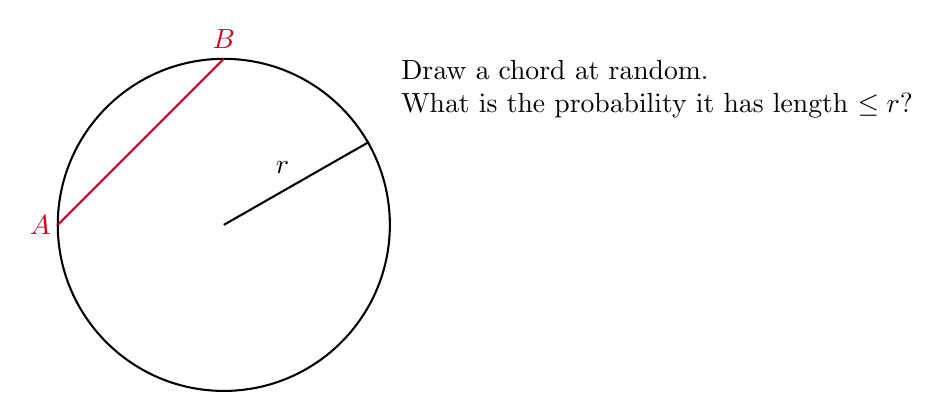
\begin{tikzpicture}[x=0.75pt,y=0.75pt,yscale=-1,xscale=1]
%uncomment if require: \path (0,300); %set diagram left start at 0, and has height of 300

%Shape: Circle [id:dp8304035694970975] 
\draw   (190,150) .. controls (190,105.82) and (225.82,70) .. (270,70) .. controls (314.18,70) and (350,105.82) .. (350,150) .. controls (350,194.18) and (314.18,230) .. (270,230) .. controls (225.82,230) and (190,194.18) .. (190,150) -- cycle ;
%Straight Lines [id:da8169764884521948] 
\draw [color={rgb, 255:red, 208; green, 2; blue, 27 }  ,draw opacity=1 ]   (190,150) -- (270,70) ;
%Straight Lines [id:da7681251331249104] 
\draw    (270,150) -- (340,110) ;

% Text Node
\draw (188,150) node [anchor=east] [inner sep=0.75pt]  [color={rgb, 255:red, 208; green, 2; blue, 27 }  ,opacity=1 ]  {$A$};
% Text Node
\draw (270,66.6) node [anchor=south] [inner sep=0.75pt]  [color={rgb, 255:red, 208; green, 2; blue, 27 }  ,opacity=1 ]  {$B$};
% Text Node
\draw (303,126.6) node [anchor=south east] [inner sep=0.75pt]    {$r$};
% Text Node
\draw (354,69) node [anchor=north west][inner sep=0.75pt]   [align=left] {Draw a chord at random.\\What is the probability it has length $\displaystyle \leq r$?};


\end{tikzpicture}\\
\nth{1} interpretation: Let $X\sim U[0,r]$\\


\tikzset{every picture/.style={line width=0.75pt}} %set default line width to 0.75pt        

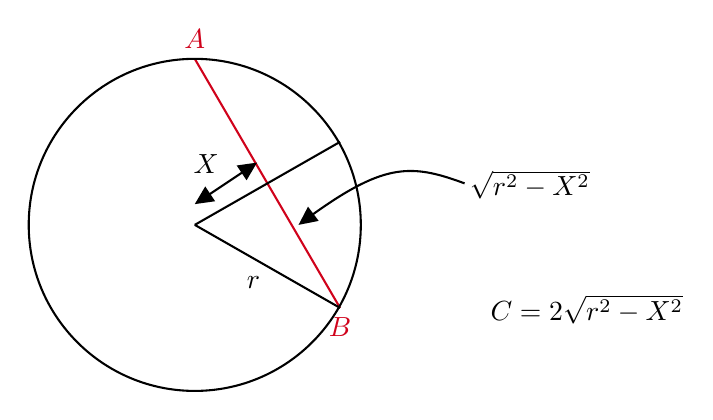
\begin{tikzpicture}[x=0.75pt,y=0.75pt,yscale=-1,xscale=1]
%uncomment if require: \path (0,300); %set diagram left start at 0, and has height of 300

%Straight Lines [id:da2699064632942776] 
\draw [color={rgb, 255:red, 208; green, 2; blue, 27 }  ,draw opacity=1 ]   (340,190) -- (270,70) ;
%Shape: Circle [id:dp6930533382122357] 
\draw   (190,150) .. controls (190,105.82) and (225.82,70) .. (270,70) .. controls (314.18,70) and (350,105.82) .. (350,150) .. controls (350,194.18) and (314.18,230) .. (270,230) .. controls (225.82,230) and (190,194.18) .. (190,150) -- cycle ;
%Straight Lines [id:da8495782823573204] 
\draw    (270,150) -- (340,110) ;
%Straight Lines [id:da5334650496901878] 
\draw    (270,150) -- (340,190) ;
%Straight Lines [id:da2034058227111022] 
\draw    (272.5,138.34) -- (297.5,121.66) ;
\draw [shift={(300,120)}, rotate = 506.31] [fill={rgb, 255:red, 0; green, 0; blue, 0 }  ][line width=0.08]  [draw opacity=0] (8.93,-4.29) -- (0,0) -- (8.93,4.29) -- cycle    ;
\draw [shift={(270,140)}, rotate = 326.31] [fill={rgb, 255:red, 0; green, 0; blue, 0 }  ][line width=0.08]  [draw opacity=0] (8.93,-4.29) -- (0,0) -- (8.93,4.29) -- cycle    ;
%Curve Lines [id:da7075937971324031] 
\draw    (322.95,147.81) .. controls (360.66,120.01) and (373.68,120.25) .. (400,130) ;
\draw [shift={(320,150)}, rotate = 323.13] [fill={rgb, 255:red, 0; green, 0; blue, 0 }  ][line width=0.08]  [draw opacity=0] (8.93,-4.29) -- (0,0) -- (8.93,4.29) -- cycle    ;

% Text Node
\draw (340,193.4) node [anchor=north] [inner sep=0.75pt]  [color={rgb, 255:red, 208; green, 2; blue, 27 }  ,opacity=1 ]  {$B$};
% Text Node
\draw (270,66.6) node [anchor=south] [inner sep=0.75pt]  [color={rgb, 255:red, 208; green, 2; blue, 27 }  ,opacity=1 ]  {$A$};
% Text Node
\draw (303,173.4) node [anchor=north east] [inner sep=0.75pt]    {$r$};
% Text Node
\draw (411,182.4) node [anchor=north west][inner sep=0.75pt]    {$C=2\sqrt{r^{2} -X^{2}}$};
% Text Node
\draw (283,126.6) node [anchor=south east] [inner sep=0.75pt]    {$X$};
% Text Node
\draw (401,122.4) node [anchor=north west][inner sep=0.75pt]    {$\sqrt{r^{2} -X^{2}}$};


\end{tikzpicture}\\
Let $C = |AB|$. What is $\mathbb{P}(C\leq r)$?\\
\[C = 2\sqrt{r^2-X^2}\]
\begin{align*}
    \mathbb{P}(C\leq r) &= \mathbb{P}(2\sqrt{r^2 - X^2}\leq r)\\
    &=\mathbb{P}(4(r^2 - X^2) \leq r^2)\\
    &=\mathbb{P}(4X^2 \geq 3r^2)\\
    &=\mathbb{P}(X\geq \sqrt{3}3/2)\\
    &=1-\frac{\sqrt{3}}{2}\\
    &\approx 0.134
\end{align*}
\end{example}
\begin{example}[cont.]
\nth{2} interpretation: Let $\theta \sim [0,2\pi]$\\
Let $C = |AB|$\\
If $\theta \in [0,\pi]$:


\tikzset{every picture/.style={line width=0.75pt}} %set default line width to 0.75pt        

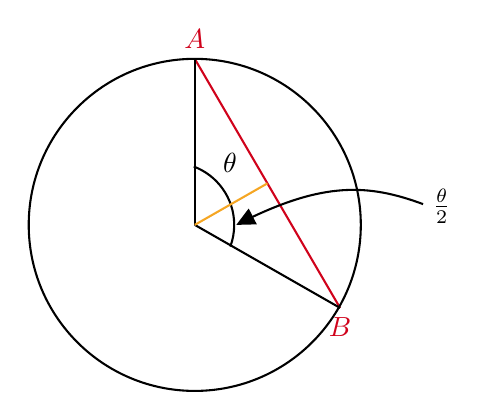
\begin{tikzpicture}[x=0.75pt,y=0.75pt,yscale=-1,xscale=1]
%uncomment if require: \path (0,300); %set diagram left start at 0, and has height of 300

%Straight Lines [id:da9970062340426395] 
\draw [color={rgb, 255:red, 208; green, 2; blue, 27 }  ,draw opacity=1 ]   (340,190) -- (270,70) ;
%Shape: Circle [id:dp8042397245788102] 
\draw   (190,150) .. controls (190,105.82) and (225.82,70) .. (270,70) .. controls (314.18,70) and (350,105.82) .. (350,150) .. controls (350,194.18) and (314.18,230) .. (270,230) .. controls (225.82,230) and (190,194.18) .. (190,150) -- cycle ;
%Straight Lines [id:da5180460606514659] 
\draw    (270,150) -- (340,190) ;
%Straight Lines [id:da39394226461044246] 
\draw    (270,150) -- (270,70) ;
%Shape: Arc [id:dp33954368677916924] 
\draw  [draw opacity=0] (269.54,121.9) .. controls (280.91,126.17) and (289,137.14) .. (289,150) .. controls (289,153.68) and (288.34,157.2) .. (287.13,160.45) -- (259,150) -- cycle ; \draw   (269.54,121.9) .. controls (280.91,126.17) and (289,137.14) .. (289,150) .. controls (289,153.68) and (288.34,157.2) .. (287.13,160.45) ;
%Straight Lines [id:da44959511705226274] 
\draw [color={rgb, 255:red, 245; green, 166; blue, 35 }  ,draw opacity=1 ]   (270,150) -- (305,130) ;
%Curve Lines [id:da9173353596556324] 
\draw    (293.04,148.47) .. controls (332.1,129.06) and (353.68,130.25) .. (380,140) ;
\draw [shift={(290,150)}, rotate = 332.88] [fill={rgb, 255:red, 0; green, 0; blue, 0 }  ][line width=0.08]  [draw opacity=0] (8.93,-4.29) -- (0,0) -- (8.93,4.29) -- cycle    ;

% Text Node
\draw (340,193.4) node [anchor=north] [inner sep=0.75pt]  [color={rgb, 255:red, 208; green, 2; blue, 27 }  ,opacity=1 ]  {$B$};
% Text Node
\draw (270,66.6) node [anchor=south] [inner sep=0.75pt]  [color={rgb, 255:red, 208; green, 2; blue, 27 }  ,opacity=1 ]  {$A$};
% Text Node
\draw (287,120) node    {$\theta $};
% Text Node
\draw (389,141) node    {$\frac{\theta }{2}$};


\end{tikzpicture}\\
\[C = 2r\sin\frac{\theta}{2}\]
If $\theta \in [\pi,2\pi]$:


\tikzset{every picture/.style={line width=0.75pt}} %set default line width to 0.75pt        

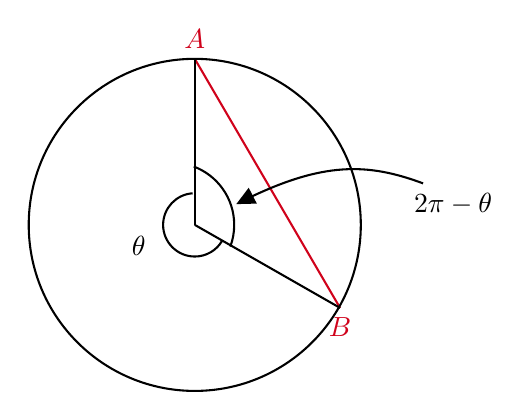
\begin{tikzpicture}[x=0.75pt,y=0.75pt,yscale=-1,xscale=1]
%uncomment if require: \path (0,300); %set diagram left start at 0, and has height of 300

%Straight Lines [id:da6345281622079197] 
\draw [color={rgb, 255:red, 208; green, 2; blue, 27 }  ,draw opacity=1 ]   (340,190) -- (270,70) ;
%Shape: Circle [id:dp610552400659343] 
\draw   (190,150) .. controls (190,105.82) and (225.82,70) .. (270,70) .. controls (314.18,70) and (350,105.82) .. (350,150) .. controls (350,194.18) and (314.18,230) .. (270,230) .. controls (225.82,230) and (190,194.18) .. (190,150) -- cycle ;
%Straight Lines [id:da2871480545724008] 
\draw    (270,150) -- (340,190) ;
%Straight Lines [id:da13010870875045866] 
\draw    (270,150) -- (270,70) ;
%Shape: Arc [id:dp08824509305722161] 
\draw  [draw opacity=0] (269.54,121.9) .. controls (280.91,126.17) and (289,137.14) .. (289,150) .. controls (289,153.68) and (288.34,157.2) .. (287.13,160.45) -- (259,150) -- cycle ; \draw   (269.54,121.9) .. controls (280.91,126.17) and (289,137.14) .. (289,150) .. controls (289,153.68) and (288.34,157.2) .. (287.13,160.45) ;
%Shape: Arc [id:dp2962628121025739] 
\draw  [draw opacity=0] (283.08,157.85) .. controls (280.41,162.28) and (275.55,165.25) .. (270,165.25) .. controls (261.58,165.25) and (254.75,158.42) .. (254.75,150) .. controls (254.75,141.92) and (261.04,135.3) .. (268.99,134.78) -- (270,150) -- cycle ; \draw   (283.08,157.85) .. controls (280.41,162.28) and (275.55,165.25) .. (270,165.25) .. controls (261.58,165.25) and (254.75,158.42) .. (254.75,150) .. controls (254.75,141.92) and (261.04,135.3) .. (268.99,134.78) ;
%Curve Lines [id:da4825449684037453] 
\draw    (293.04,138.47) .. controls (332.1,119.06) and (353.68,120.25) .. (380,130) ;
\draw [shift={(290,140)}, rotate = 332.88] [fill={rgb, 255:red, 0; green, 0; blue, 0 }  ][line width=0.08]  [draw opacity=0] (8.93,-4.29) -- (0,0) -- (8.93,4.29) -- cycle    ;

% Text Node
\draw (340,193.4) node [anchor=north] [inner sep=0.75pt]  [color={rgb, 255:red, 208; green, 2; blue, 27 }  ,opacity=1 ]  {$B$};
% Text Node
\draw (270,66.6) node [anchor=south] [inner sep=0.75pt]  [color={rgb, 255:red, 208; green, 2; blue, 27 }  ,opacity=1 ]  {$A$};
% Text Node
\draw (243,160) node    {$\theta $};
% Text Node
\draw (394.5,140) node    {$2\pi -\theta $};


\end{tikzpicture}\\
\[C = 2r\sin\frac{2\pi - \theta}{2} = 2r\sin\frac{\theta}{2}\]
\begin{align*}
    \mathbb{P}(C\leq r) &= \mathbb{P}(2r\sin\frac{\theta}{2}\leq r)\\
    &= \mathbb{P}(\sin\frac{\theta}{2}\leq \frac{1}{2})\\
    &=\mathbb{P}(\theta\leq \frac{\pi}{3}) + \mathbb{P}(\theta\geq \frac{\pi}{3})\\
    &=\frac{1}{6}+\frac{1}{6}\\
    &=\frac{1}{3}\\
    &\approx 0.333\dots
\end{align*}
\end{example}

\subsection{Buffon's Needle}
\begin{example}

\hfill{ }\\
\tikzset{every picture/.style={line width=0.75pt}} %set default line width to 0.75pt        

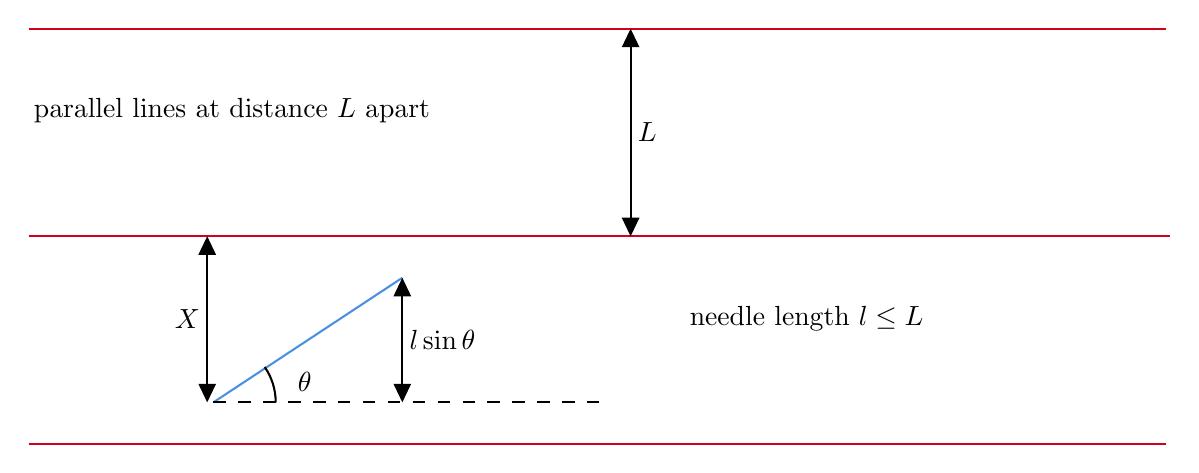
\begin{tikzpicture}[x=0.75pt,y=0.75pt,yscale=-1,xscale=1]
%uncomment if require: \path (0,471); %set diagram left start at 0, and has height of 471

%Straight Lines [id:da997608533938259] 
\draw [color={rgb, 255:red, 208; green, 2; blue, 27 }  ,draw opacity=1 ]   (30,140) -- (580,140) ;
%Straight Lines [id:da9529405542542617] 
\draw [color={rgb, 255:red, 208; green, 2; blue, 27 }  ,draw opacity=1 ]   (30,40) -- (578,40) ;
%Straight Lines [id:da08762779844726043] 
\draw [color={rgb, 255:red, 208; green, 2; blue, 27 }  ,draw opacity=1 ]   (30,240) -- (578,240) ;
%Straight Lines [id:da5819554456791083] 
\draw    (320,43) -- (320,137) ;
\draw [shift={(320,140)}, rotate = 270] [fill={rgb, 255:red, 0; green, 0; blue, 0 }  ][line width=0.08]  [draw opacity=0] (8.93,-4.29) -- (0,0) -- (8.93,4.29) -- cycle    ;
\draw [shift={(320,40)}, rotate = 90] [fill={rgb, 255:red, 0; green, 0; blue, 0 }  ][line width=0.08]  [draw opacity=0] (8.93,-4.29) -- (0,0) -- (8.93,4.29) -- cycle    ;
%Straight Lines [id:da6866039754162403] 
\draw [color={rgb, 255:red, 74; green, 144; blue, 226 }  ,draw opacity=1 ]   (210,160) -- (119,220) ;
%Shape: Arc [id:dp8703968059678213] 
\draw  [draw opacity=0] (143.72,203) .. controls (147.05,207.83) and (149,213.69) .. (149,220) -- (119,220) -- cycle ; \draw   (143.72,203) .. controls (147.05,207.83) and (149,213.69) .. (149,220) ;
%Straight Lines [id:da5603174559367186] 
\draw    (116,143) -- (116,217) ;
\draw [shift={(116,220)}, rotate = 270] [fill={rgb, 255:red, 0; green, 0; blue, 0 }  ][line width=0.08]  [draw opacity=0] (8.93,-4.29) -- (0,0) -- (8.93,4.29) -- cycle    ;
\draw [shift={(116,140)}, rotate = 90] [fill={rgb, 255:red, 0; green, 0; blue, 0 }  ][line width=0.08]  [draw opacity=0] (8.93,-4.29) -- (0,0) -- (8.93,4.29) -- cycle    ;
%Straight Lines [id:da9696993051458238] 
\draw  [dash pattern={on 4.5pt off 4.5pt}]  (119,220) -- (310,220) ;
%Straight Lines [id:da40517689204938323] 
\draw    (210,163) -- (210,217) ;
\draw [shift={(210,220)}, rotate = 270] [fill={rgb, 255:red, 0; green, 0; blue, 0 }  ][line width=0.08]  [draw opacity=0] (8.93,-4.29) -- (0,0) -- (8.93,4.29) -- cycle    ;
\draw [shift={(210,160)}, rotate = 90] [fill={rgb, 255:red, 0; green, 0; blue, 0 }  ][line width=0.08]  [draw opacity=0] (8.93,-4.29) -- (0,0) -- (8.93,4.29) -- cycle    ;

% Text Node
\draw (322,90) node [anchor=west] [inner sep=0.75pt]    {$L$};
% Text Node
\draw (163,210) node    {$\theta $};
% Text Node
\draw (114,180) node [anchor=east] [inner sep=0.75pt]    {$X$};
% Text Node
\draw (212,190) node [anchor=west] [inner sep=0.75pt]    {$l\sin \theta $};
% Text Node
\draw (31,72) node [anchor=north west][inner sep=0.75pt]  [color={rgb, 255:red, 0; green, 0; blue, 0 }  ,opacity=1 ] [align=left] {parallel lines at distance $\displaystyle L$ apart};
% Text Node
\draw (347,172) node [anchor=north west][inner sep=0.75pt]  [color={rgb, 255:red, 0; green, 0; blue, 0 }  ,opacity=1 ] [align=left] {needle length $\displaystyle l\leq L$};


\end{tikzpicture}\\
Throw the needle at random. What is the probability it intersects at least one line?
\[\theta \sim U[0,\pi], \ X \sim U[0,L]\text{ indep.}\]
It intersects a line iff $X\leq l\sin\theta$.
\[\mathbb{P}(\text{intersection}) = \mathbb{P} (X\leq l\sin\theta) = \int_0^L\int_0^{\pi}\frac{1}{\pi L} 1(x\leq l\sin\theta)\,\dd x\,\dd \theta = \frac{2l}{\pi L}\]
So $p = \frac{2l}{\pi L}$
\[\implies\pi = \frac{2l}{pL}\]
Want to use this experiment to approximate $\pi$. Throw $n$ needles indep. and let $\hat{p}_n$ be the proportion intersecting a line. Then $\hat{p}_n$ approximates $p$ and so
\[\hat{\pi}_n = \frac{2l}{\hat{p}_n}L\text{ approximates }\pi\]
Suppose
\[\mathbb{P}(|\hat{\pi}_n - \pi|\leq 0.001) \geq 0.99\]
How large should $n$ be?
\end{example}
\begin{example}[cont.]


$S_n =$ number of needles intersecting a line
\[S_n \sim \text{ Bin}(n,p)\]
By the CLT, $S_n \sim np + \sqrt{np(1-p)}\cdot Z, Z\sim N(0,1)$
\[\hat{p}_n  = \frac{S_n}{n} \approx p + \sqrt{\frac{p(1-p)}{n}}\cdot Z\]
So
\[\hat{p}_n- p \approx \sqrt{\frac{p(1-p)}{n}}\cdot \]
Define $f(x) = \frac{2l}{xL}$. Then $f(p) = \pi$ and $f'(p) = -\pi/p$ and $\hat{\pi}_n= f(\hat{p}_n)$.\\
By Taylor expansion, $\hat{\pi}_n = f(\hat{p}_n) \approx f(p) + (\hat{p}_n - p)f'(p)$
\[\implies\hat{\pi}_n\approx \pi - (\hat{p}_n    - p) \cdot\frac{\pi}{p}\]
\[\implies\hat{\pi}_n - \pi\approx -\frac{\pi}{p}\sqrt{\frac{p(1-p)}{n}} = -\pi \sqrt{\frac{1-p}{pn}}\cdot Z\]
We want
\[\mathbb{P}\left(\pi\sqrt{\frac{1-p}{pn}} \cdot |Z| \leq 0.001\right) \geq 0.99\]
Have $\mathbb{P}(|Z|\geq 2.58) = 0.01$ and $\pi^2 \cdot \frac{1-p}{pn}$ decreasing in $p$. Minimise $\pi^2 \cdot \frac{1-p}{pn}$ by taking $l = L \implies p = \frac{2}{\pi}$ and 
\[\v = \frac{\pi^2}{n} \left(\frac{\pi}{2} - 1\right)\]
Taking
\[\sqrt{\frac{\pi^2}{n} \left(\frac{\pi}{2} - 1\right)} \cdot 2.58 = 0.001 \implies n = 3.75\times 10^7\]

\end{example}